\chapter{Modelling and Analysis of DVC in a Digital Twin of 66 kV HVAC Offshore Network}\label{3}

In this chapter, the basics of \gls{EMT} software utilized is explained briefly. Then the model consisting of a Type-4 \gls{WG} with implemented \gls{DVC} from \cite{korai_dynamic_2019} in a 66 kV \gls{HVAC} offshore network in RSCAD is detailed. The performance of the control strategy is tested for severe dynamic conditions. Lastly, the performance of the \gls{DVC} modelled in RSCAD is then validated with the benchmark \gls{DVC} model in DIgSILENT PowerFactory software \cite{erlich_description_2018} (based on a qualitative comparison because of the unavoidable differences between the software packages) for a similar 66 kV \gls{HVAC} offshore network.

\section{Real Time Digital Simulator (RTDS) Tool}\label{RTDS_Theory}
Real Time Digital Simulator (\gls{RTDS}) Hardware is equipped to perform \gls{EMT} simulations. The overall network solution in \gls{RTDS} is based on nodal analysis. The simulator can work in the range from \gls{DC} to 3 kHz of frequency. It can simulate a time step of 25 - 50 $\mu$s for even complex power systems. This is termed as a large time step. \gls{RTDS} gives the option for a small time step environment to incorporate \gls{PE} components simulation. These blocks have time steps in the range of 1400  - 3750 ns. The hardware consists of two generations of processor cards, namely, PB5 and NovaCor \cite{rtds_tech}.  

\gls{RTDS} provides a user-friendly Guided User Interface (GUI) called RSCAD wherein the network is modelled, run and analyzed. There are modules available in RSCAD for the actions mentioned above (Figure \ref{fig:RSCAD_modules}). These are explained in \cite{rtds_tech} in detail. The majorly used modules for this thesis are the Draft, Runtime, Cable and Tline modules. The modelling of the system is performed in the Draft module, which contains a drawing canvas whose size can be adjusted. The working of the Cable and Tline modules are illustrated in Sections \ref{HVAC_cable_RSCAD} and \ref{Tline_cable_RSCAD}, respectively. After the model is developed, the simulation is run in the Runtime module. \gls{RTDS} also allows for Hardware In Loop (HIL) and Software In Loop (SIL) simulations to test the working of controllers in real-world scenario \cite{rtds_tech_hardware}.

\begin{figure}[H]
\centering
%\hspace*{-1.2cm}
    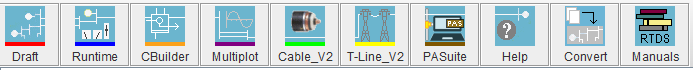
\includegraphics[height = 1.4cm,width = 14.5cm]{Diagrams/Chapter_3/RSCAD_modules.PNG}
    \caption{Modules available in RSCAD}
    \label{fig:RSCAD_modules}
\end{figure}

A simple network model in the Draft module layout is shown in Figure \ref{fig:Dft_RSCAD}. The time step, plot duration and the canvas size is assigned by right-clicking on anywhere on the canvas area and choosing the "Circuit Options" as shown in Figure \ref{fig:Dft_RSCAD}.

\begin{figure}[H]
\centering
%\hspace*{-1.2cm}
    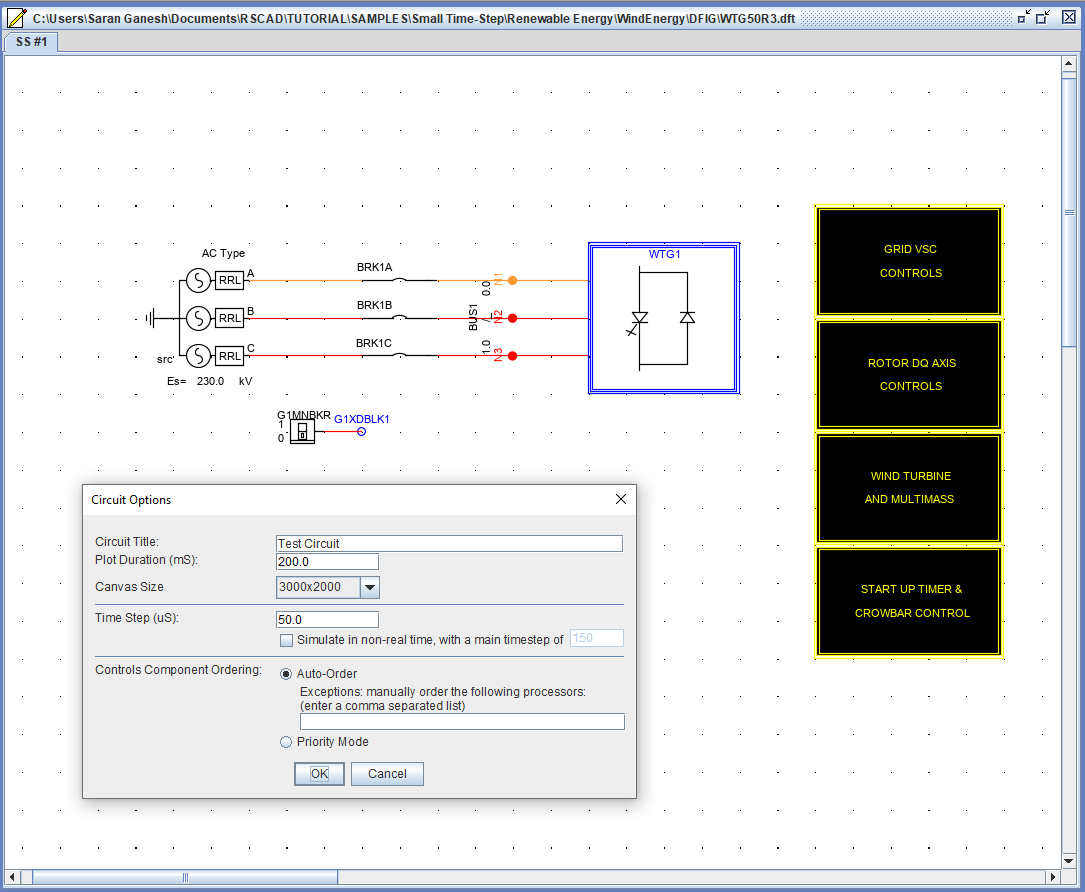
\includegraphics[height = 9cm,width = 11.5cm]{Diagrams/Chapter_3/Dft_RSCAD.PNG}
    \caption{Example of a power system in Draft module in RSCAD}
    \label{fig:Dft_RSCAD}
\end{figure}

There are different libraries available in the Draft module to select the components. The major libraries that were used are \cite{rtds_tech}:
\begin{itemize}\label{Library_RSCAD}
    \item Power system library (Figure \ref{fig:Power_system_lib}) - Consists of power component models such as transformer, transmission line, cables and so forth. These components are to be used in the large time step in the workspace. 
    \item Small time step library - This library consists of components that are used to model in the small time step environment. The mainly used components are the \gls{VSC} bridge box, \gls{VSC} interface transformers, Tline block to interface between small time step environment and large time step environment.    
    \item Controls library (Figure \ref{fig:Controls_lib}) - The most important block for modelling control strategies. Consists of transfer functions, logic functions, math functions and so forth.
\end{itemize}

\begin{figure}[H]
\centering
\begin{subfigure}{.5\textwidth}
  \centering
  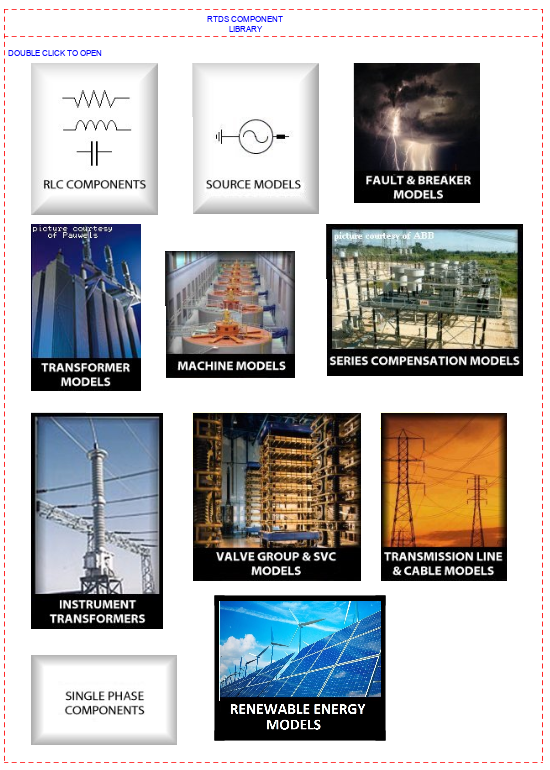
\includegraphics[height=8cm,width=7cm]{Diagrams/Chapter_3/Power_system_lib.PNG}
  \caption{Power system library in Draft module}
  \label{fig:Power_system_lib}
\end{subfigure}%
\begin{subfigure}{.5\textwidth}
  \centering
  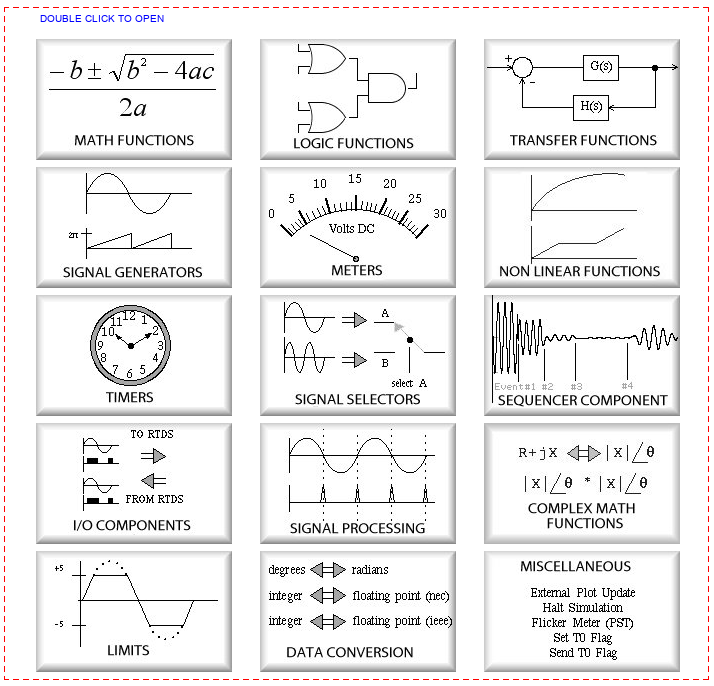
\includegraphics[height=8cm,width=8cm]{Diagrams/Chapter_3/Control_system_lib.PNG}
  \caption{Controls library in Draft module}
  \label{fig:Controls_lib}
\end{subfigure}
\caption{Libraries available in Draft module in RSCAD}
%\label{fig:test}
\end{figure}

After the model has been developed in the Draft module as shown in Figure \ref{fig:Dft_RSCAD}, the user has to compile the file by clicking on "Compile" \footnote{Compile icon in RSCAD: 
\includegraphics[width=0.6cm, height=0.6cm]{Diagrams/Chapter_3/Compile_pic.PNG}}. The processor calculates the actual time step, and the initial conditions are stored in the MAP file which is available by right-clicking on the white space in the draft module. The user is notified of errors or warnings during simulation through a pop-up box at the end of file compilation. The processor assignment and the controls assignment can be viewed by clicking the "Processor Assignment" \footnote{Processor Assignment icon in RSCAD 
\includegraphics[width=0.6cm, height=0.6cm]{Diagrams/Chapter_3/Processor_assignment_pic.PNG}} tab. There are some important data in the RSCAD configuration files that hold information about the configuration of hardware in \gls{RTDS}. IP addresses of all rack ports and the processor cards are the data available in the configuration file. It can be accessed using the "Tool" menu in the main tab of RSCAD. Improper configuration of these files will result in no simulation of the test case \cite{rtds_tech}. 

The real-time interaction of the user with the system is done through the Runtime module available in RSCAD. The user can accomplish tasks like measuring signals, plotting graphs, adjusting sliders and creating faults in this interface. An example of the Runtime module with the scenarios mentioned above is shown in Figure \ref{fig:Runtime_RSCAD}.

\begin{figure}[H]
\centering
%\hspace*{-1.2cm}
    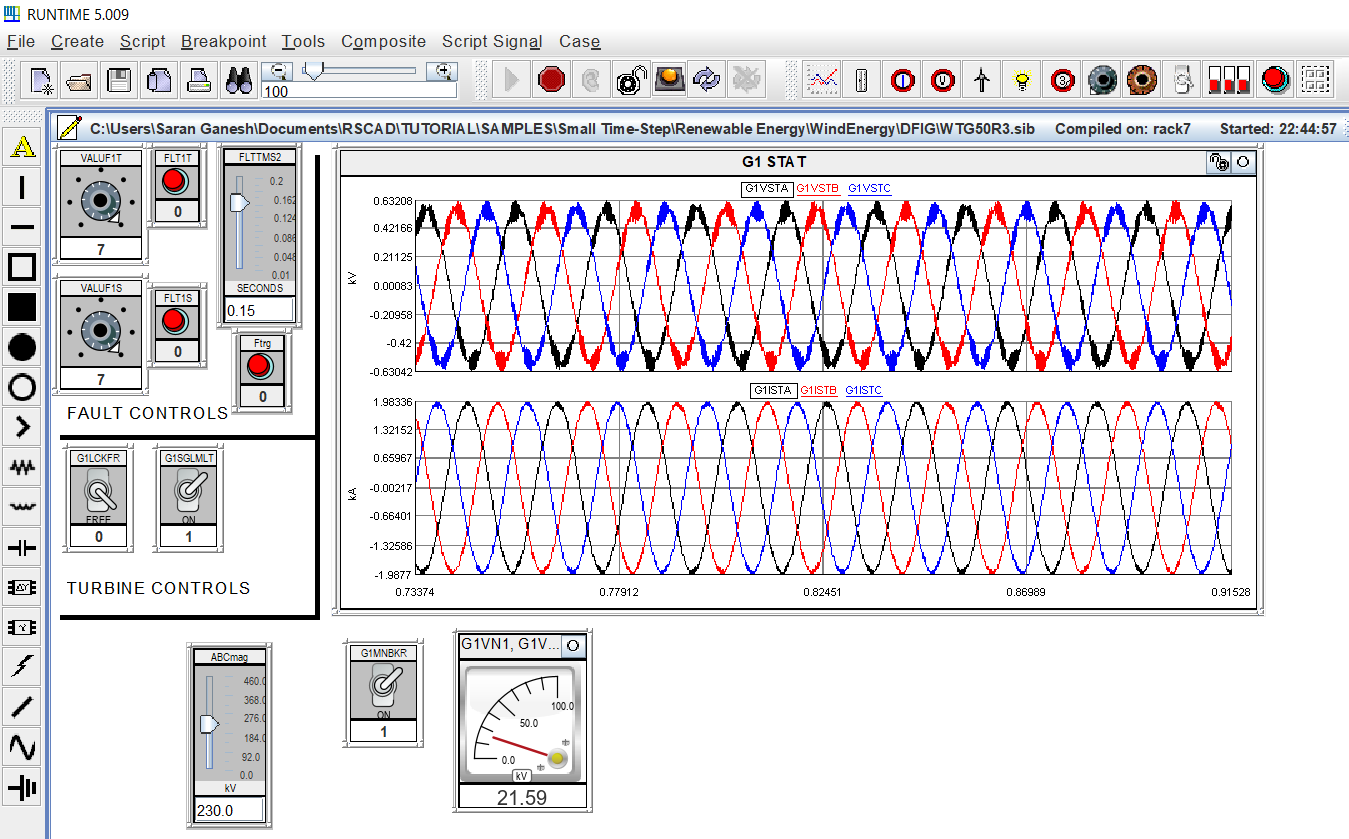
\includegraphics[height = 12cm,width = \textwidth]{Diagrams/Chapter_3/Runtime_pic.PNG}
    \caption{Example of the Runtime module with plots, switches, sliders etc. in RSCAD}
    \label{fig:Runtime_RSCAD}
\end{figure}



The overall working of RSCAD can be understood as depicted by the flowchart in Figure \ref{fig:RSCAD_Flowchart}.
\begin{figure}[H]
\centering
%\hspace*{-2.1cm}
    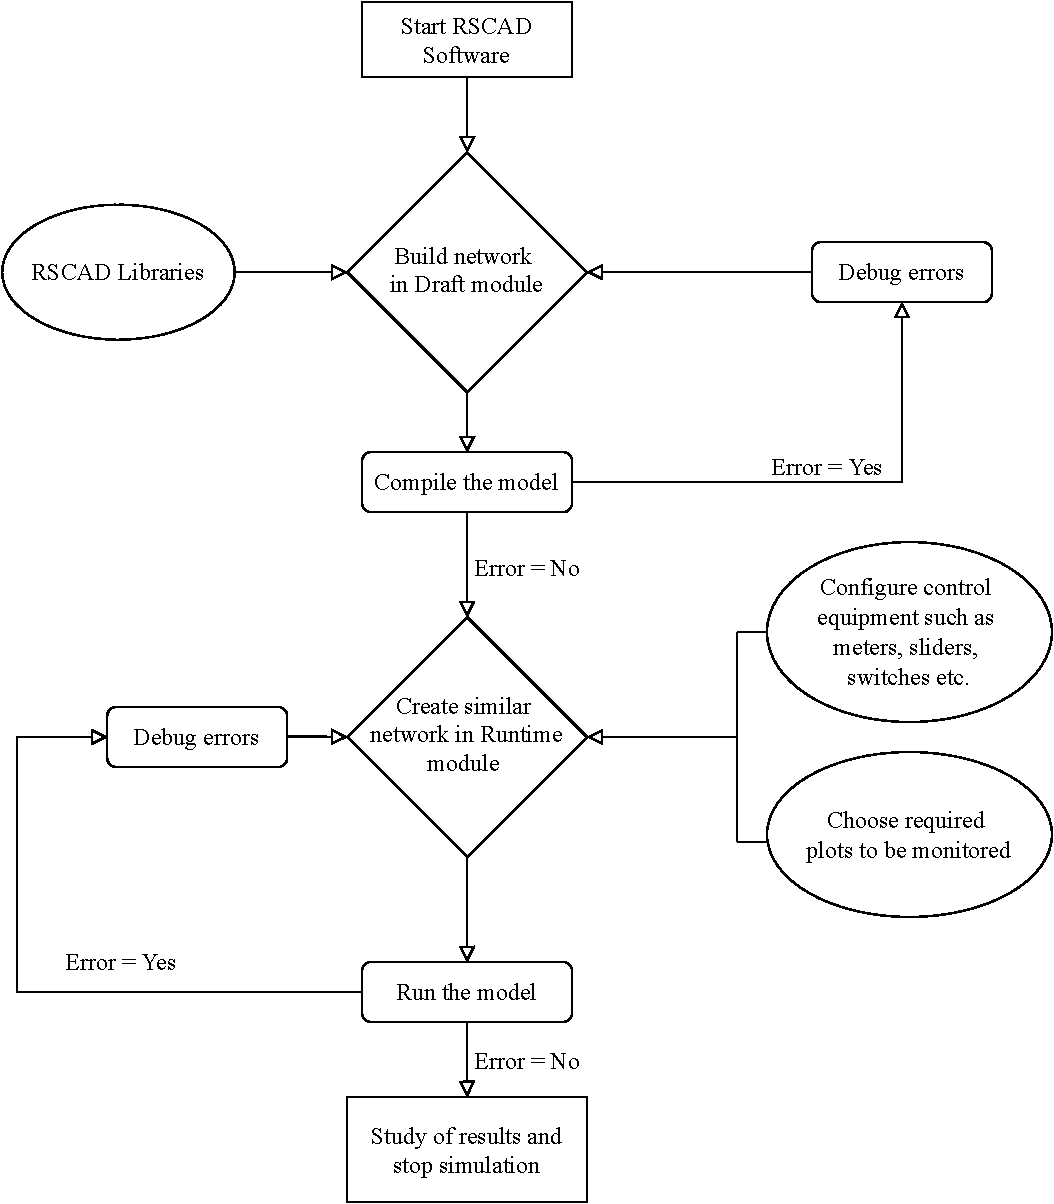
\includegraphics[height = 14.5cm,width = 12.5cm]{Diagrams/Chapter_3/RSCAD_Flowchart.pdf}
    \caption{Flowchart representation of RSCAD working}
    \label{fig:RSCAD_Flowchart}
\end{figure}

\section{Layout of the 66 kV HVAC Test System in RSCAD}\label{RSCAD_ACsourcemodel}\label{WT1_ACsource_RSCAD_Test_Layout}
After understanding the basics of RSCAD software, a 66 kV offshore network, as shown in Figure \ref{fig:WT1_Model_RSCAD} is developed. The network consists of the following components.

\begin{itemize}
    \item An aggregated representation of 700 MW installed capacity Offshore Wind Farm (\gls{OWF}) is modelled with the following elements:
    \begin{itemize}
        \item A single Wind Generation System with 
    \begin{itemize}
        \item Permanent Magnet Synchronous Generator (\gls{PMSG})
        \item Machine Side Converter (\gls{MSC})
        \item \gls{DC} circuit
        \item Grid Side Converter (\gls{GSC}) 
    \end{itemize}
        \item High Pass filter (\gls{HPF}) with series reactor
        \item \gls{OWF} transformer
    \end{itemize}
    \item \gls{HVAC} cables  
     \item External \gls{AC} system
\end{itemize}

\begin{figure}[H]
\centering
%\hspace*{-1cm}
    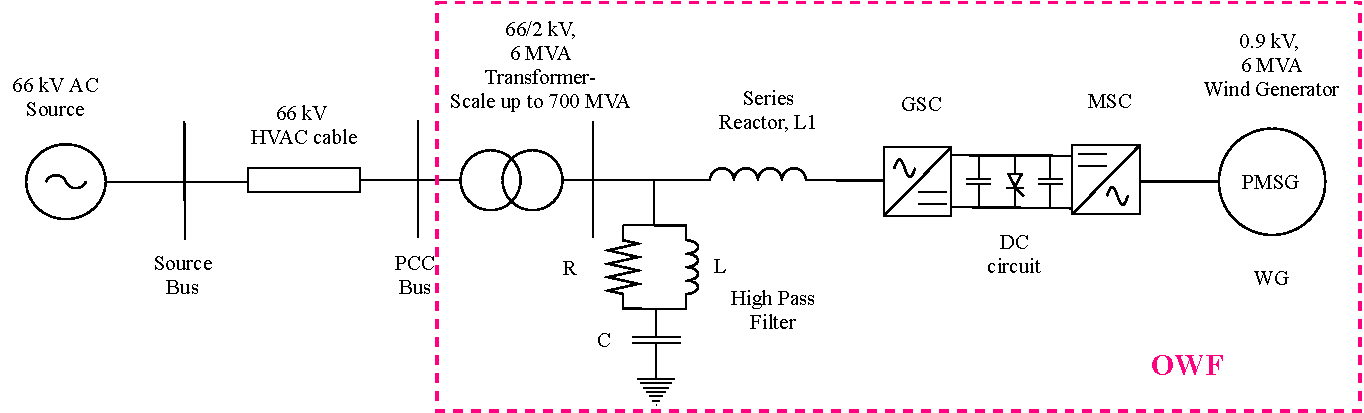
\includegraphics[height = 5.5cm,width = \textwidth]{Diagrams/Chapter_3/WT1_AC_RSCAD_OWF.pdf}
    \caption{Single line diagram of the 66 kV HVAC offshore test network in RSCAD}
    \label{fig:WT1_Model_RSCAD}
\end{figure}

\subsection{ Aggregated Offshore Wind farm (OWF)}\label{OWF}

The 700 MW offshore wind power is represented by a single \gls{OWF} consisting of 116 \gls{WG}s, each rated 6 MW connected in parallel. Type-4 \gls{WG}s are used for all units. The RSCAD representation of aggregated \gls{OWF} is utilized in this work. The aggregated model consists of \gls{PE} components which require high switching frequency %(19*50 = 950 Hz in this case) 
and hence is modelled in a small time step environment by selecting the "VSC Bridge Box" (Figure \ref{fig:SmallTimeStepBlock}) available in the small time step library in the Draft module. The box contains the \gls{PMSG}, \gls{MSC}, \gls{DC} capacitors, chopper circuit, \gls{GSC}, \gls{HPF} with series reactor and \gls{OWF} transformer as illustrated in Figure \ref{fig:OveriewSmallTimeStepOWF}. As mentioned in Section \ref{RTDS_Theory}, the block can be assigned to have a time step value between 1400 to 3750 ns. Hence, a value of 2500 ns is chosen for this model. 
%It is necessary to set this time step to a nearly high value to avoid the time step overflow error in RSCAD.
The value can be entered by right-clicking on the small time step block and choosing "Edit" and then "Parameters" as shown in Figure \ref{fig:SmallTimeStepBlock}. Also, it must the noted that the above-specified time step is only for initialization and the actual used time step can be viewed in the Map file which is accessible by right-clicking on any white space in the Draft file and selecting "View" then, "Map File". It is also worth mentioning that the ratio of the large time step to the small-time step in a network in RSCAD must be higher than 12 when using NovaCor and must be higher than 17 when using PB5 racks \cite{rtds_tech}. 

\begin{figure}[H]
\centering
%\hspace*{-4.2cm}
    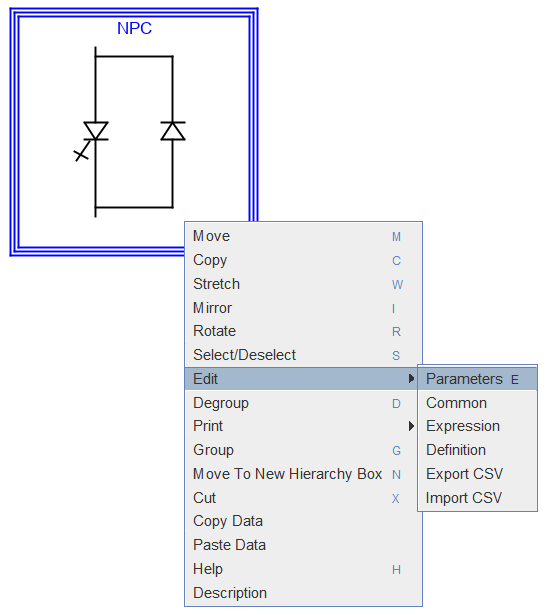
\includegraphics[height = 8cm,width = 7cm]{Diagrams/Chapter_3/SmallTimeStepBlock.PNG}
    \caption{Small time step block}
    \label{fig:SmallTimeStepBlock}
\end{figure}

\subsubsection{Wind Generation System}
The wind generation system consists of \gls{PMSG}, \gls{MSC}, \gls{DC} circuit and \gls{GSC}. The \gls{EMT} model of Type-4 \gls{WG} with detailed modelling of \gls{MSC}, \gls{DC} circuit and \gls{GSC} represented by three-level \gls{VSC}s are utilized for this work. The basic models for this work are considered from the MIGRATE project \cite{denis_migrate_2018}. The detailed description of the \gls{PMSG}, \gls{MSC} and \gls{DC} circuit models along with the control structures are explained in Appendix \ref{Appendix_A}. The control for \gls{GSC} developed in \cite{sethi_real-time_nodate-new} is modified and implemented in this thesis work. This is explained in detail in Section \ref{DVC_RSCAD}.

\begin{figure}[H]
\text{\rotatebox{90}{\hspace{5mm}
\noindent
{\color{magenta} \rule{10mm}{1mm} } \gls{OWF} Transformer
\hspace{15mm}
\noindent
{\color{blue} \rule{10mm}{1mm} } \gls{HPF} with reactor
\hspace{15mm}
\noindent
{\color{green} \rule{10mm}{1mm} } \gls{GSC}
\hspace{15mm}
\noindent
{\color{orange} \rule{10mm}{1mm} } DC Circuit
\hspace{15mm}
\noindent
{\color{yellow} \rule{10mm}{1mm} } \gls{MSC}
\hspace{15mm}
\noindent
{\color{violet} \rule{10mm}{1mm} } \gls{PMSG}}
}
\hspace{10mm}
\centering
%\hspace*{-1.2cm}
    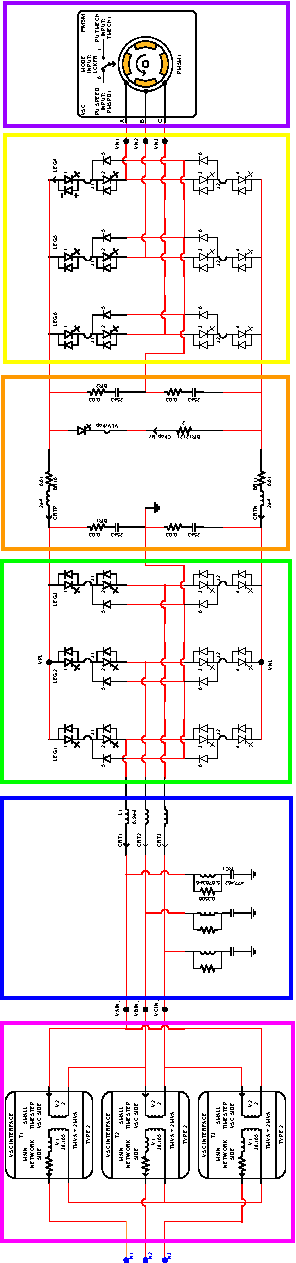
\includegraphics[height = 25cm,width = 6cm]{Diagrams/Chapter_3/SmallTimeStep_WTModel_New3.pdf}
    \caption{Overview of OWF model in small time step environment}
    \label{fig:OveriewSmallTimeStepOWF}
\end{figure}


\subsubsection{High Pass Filter (HPF) with Series Reactor}\label{HPF_design}
The switching operation of \gls{PE} converters leads to generation of harmonics. Thereby, to mitigate these harmonics, filters are provided at the output of the \gls{GSC}. There are various types of filters available for this application. The common ones are the LCL filter, L filter and high pass filter \cite{beres_review_2016}. In RSCAD, there is a \gls{HPF} block readily available in the small time step library, as shown in Figure \ref{fig:HPF} \cite{rtds_tech}. It is chosen by selecting the \gls{VSC} branch model in this library and changing the branch type to "HIPASS". A three-phase inductance branch is chosen by selecting the branch type to "L" and connected as the series reactor, as depicted in the blue box in Figure \ref{fig:OveriewSmallTimeStepOWF}. After the \gls{HPF} parameters are calculated and set, then it would only be required to tune the inductance of the series reactor to limit the flow of current and thereby stabilizing the voltage. Hence, it was decided to go with \gls{HPF}.

\begin{figure}[H]
\centering
%\hspace*{-4.2cm}
    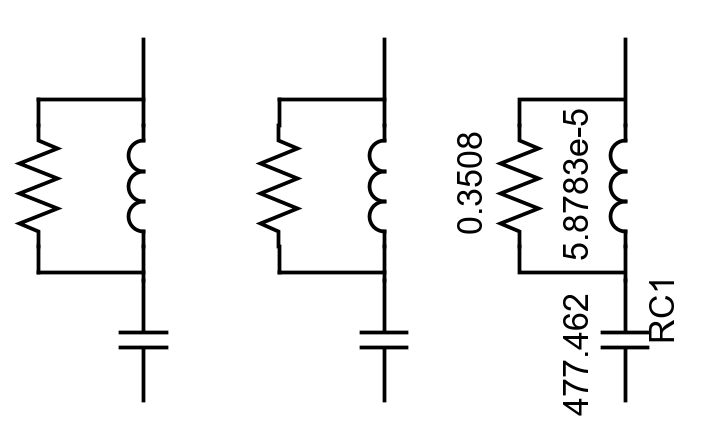
\includegraphics[height = 3.5cm,width = 5cm]{Diagrams/Chapter_3/HPF_RSCAD.PNG}
    \caption{High Pass Filter in RSCAD}
    \label{fig:HPF}
\end{figure}

The base impedance on the low voltage side of transformer is calculated in ohms as in Equation \ref{base_impedance}.
\begin{equation}\label{base_impedance}
    Z_{baseLV} = \frac{LV^2}{Base MVA} = \frac{(2 kV)^2}{6 MVA} = 0.6667\Omega  
\end{equation}

The \gls{HPF} should have a high impedance value at the nominal frequency (50 Hz) so that it works as an open circuit. Therefore, a higher value of 10 times base impedance is chosen. The impedance of the capacitor at 50 Hz is computed by the following equation.

\begin{equation}
    Z_c = 10 * Z_{baseLV} = 10 * 0.6667 \Omega = 6.667 \Omega   
\end{equation}
Hence, the value of capacitance at 50 Hz in Farad is calculated by using Equation \ref{capac_eq},
\begin{equation}\label{capac_eq}
    C = \frac{1}{2\pi f *Z_c} = \frac{1}{2\pi*50 Hz*6.667\Omega} = 4.77462*10^{-4} F
\end{equation}

The next step is to calculate the inductance 'L'. The inductance must be selected so that during the switching or modulating frequency (950 Hz in this case), the impedance of the inductor and capacitor cancel each other. The switching and higher frequencies can be passed to the ground and thereby purely sinusoidal signals will be transferred to the \gls{PCC}. The impedance of the inductor, resistor and capacitor must be equal at the switching frequency in order to pass the high frequencies to the ground. Therefore, to calculate inductance, it is considered as a series LC circuit. The resonant frequency of the LC circuit is given by Equation \ref{resosn_freq_eq}.

\begin{equation}\label{resosn_freq_eq}
    \omega = \frac{1}{\sqrt{L*C}}    
\end{equation}

Hence, the inductance value can be calculated as per the following equation.

\begin{equation}
    L = \frac{1}{\omega^2*C} = \frac{1}{(2\pi * 950 Hz)^2* 4.77462*10^{-4} F} = 5.8783*10^{-5} H
\end{equation}

Upon deriving the inductance, the resistance is selected to match the impedance of the parallel inductor at the modulating frequency.

\begin{equation}
    R = \omega* L = (2\pi*950 Hz)*5.8783*10^{-5} H = 0.3508 \Omega
\end{equation}

The series reactor is used for limiting the current to the \gls{AC} network. The inductance value of the reactor was selected after precise tuning and is set to 0.9 mH to achieve voltage of 1 p.u. at the \gls{PCC}.

\subsubsection{OWF Transformer}\label{scaling_OWF}
The \gls{GSC} is connected in series to a three-phase offshore 66/2 kV, 6 MVA transformer with leakage reactance of 10 \%, through a series reactor and a shunt \gls{HPF} as seen in Figure \ref{fig:OveriewSmallTimeStepOWF}. Single-phase \gls{VSC} interface transformer shown in Figure \ref{fig:VSC_interface_trafo_smalldt} available in the small time step library is used for this approach. Three transformers each rated 2 MVA are connected in wye-delta configuration with as seen in Figure \ref{fig:OveriewSmallTimeStepOWF}. In RSCAD, the scaling up of power is done at this transformer. The option for scaling up the primary current of the transformer is available in the \gls{VSC} interface transformer block as shown in Figure \ref{fig:VSC_interface_trafo_scaling} \cite{rtds_tech}. The user can control the amount of scaling, i.e. the number of parallel units by a slider, as shown in Figure \ref{fig:scaling_factor_RSCAD}. The user can model the components in the secondary side of the transformer as required for a single \gls{WG} and then scale it to the required power (nearly 700 MW in this case).

\begin{figure}[H]
\centering
%\hspace*{-4.2cm}
    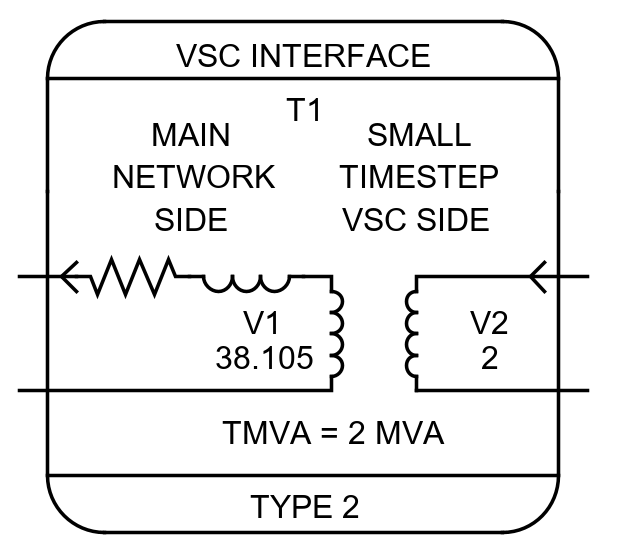
\includegraphics[height = 4cm,width = 4.5cm]{Diagrams/Chapter_3/VSC_interface_trafo_smalldt.PNG}
    \caption{VSC interface transformer}
    \label{fig:VSC_interface_trafo_smalldt}
\end{figure}
\vspace{0 mm}
\begin{figure}[H]
\centering
\begin{subfigure}{.55\textwidth}
  \centering
  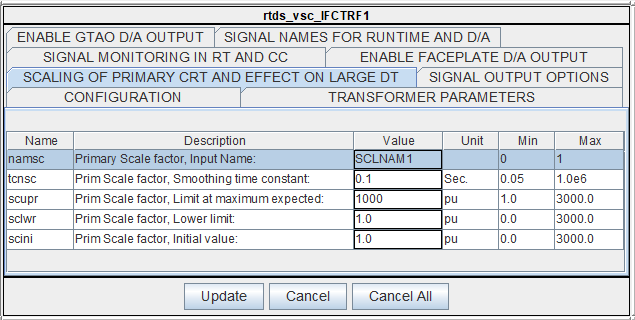
\includegraphics[height=5cm,width=10cm]{Diagrams/Chapter_3/VSC_interface_trafo_scaling.PNG}
  \caption{Option for scaling in VSC transformer}
  \label{fig:VSC_interface_trafo_scaling}
\end{subfigure}%
\begin{subfigure}{.5\textwidth}
  \centering
  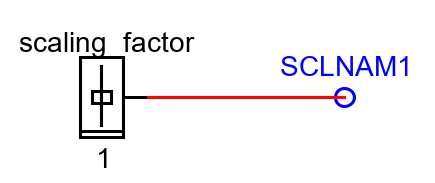
\includegraphics[height=2cm,width=4.5cm]{Diagrams/Chapter_3/scaling_factor_RSCAD.PNG}
  \caption{Scaling factor}
  \label{fig:scaling_factor_RSCAD}
\end{subfigure}
\caption{Scaling up of power in RSCAD}
\label{fig:VSC_trafo_options}
\end{figure}

\subsection{HVAC Cables}\label{HVAC_cable_RSCAD}
The \gls{HVAC} cables transfer power from the \gls{OWF} transformer to the external \gls{AC} system. The \gls{HVAC} cables are rated at 66 kV and modelled in the large time step environment. When compared to 33 kV cables, 66 kV cables allow twice the amount of power to be transferred for the same area of cross-section and require lower array cabling \cite{dnv66kv}. 
 
RSCAD allows cables to be modelled as Frequency Dependent Phase, Bergeron and Pi models \cite{rtds_tech}. The Frequency Dependent Phase and the Bergeron are travelling wave models. Pi model representation of cable is chosen for this research in RSCAD. To ease the goal of comparing the performance of models in two \gls{EMT} software, which is explained later in this chapter, a Pi cable model was chosen. In RSCAD, cable parameters can be entered using the Cable module available in the RSCAD modules section as denoted by a red box in Figure \ref{fig:CableModule_mark}. 

 
In the Draft module, the cable model is added in the circuit using the unified model shown in Figure \ref{fig:CableParaBlock} available in RSCAD power system library. The unified model consists of the following components: 
%\setlist{nolistsep}
    \begin{itemize}[noitemsep]
    \item Calculation Block
    \item Sending End Terminal
    \item Receiving End Terminal
\end{itemize}

The detailed representation of the cable parameters in Cable module, and the representation of the cable model using the calculation block, sending end terminal and receiving end terminals in the Draft module is shown in Appendix \ref{config_cable}.

%\vspace{-13mm}
\begin{figure}[H]
\centering
%\hspace*{-1.2cm}
    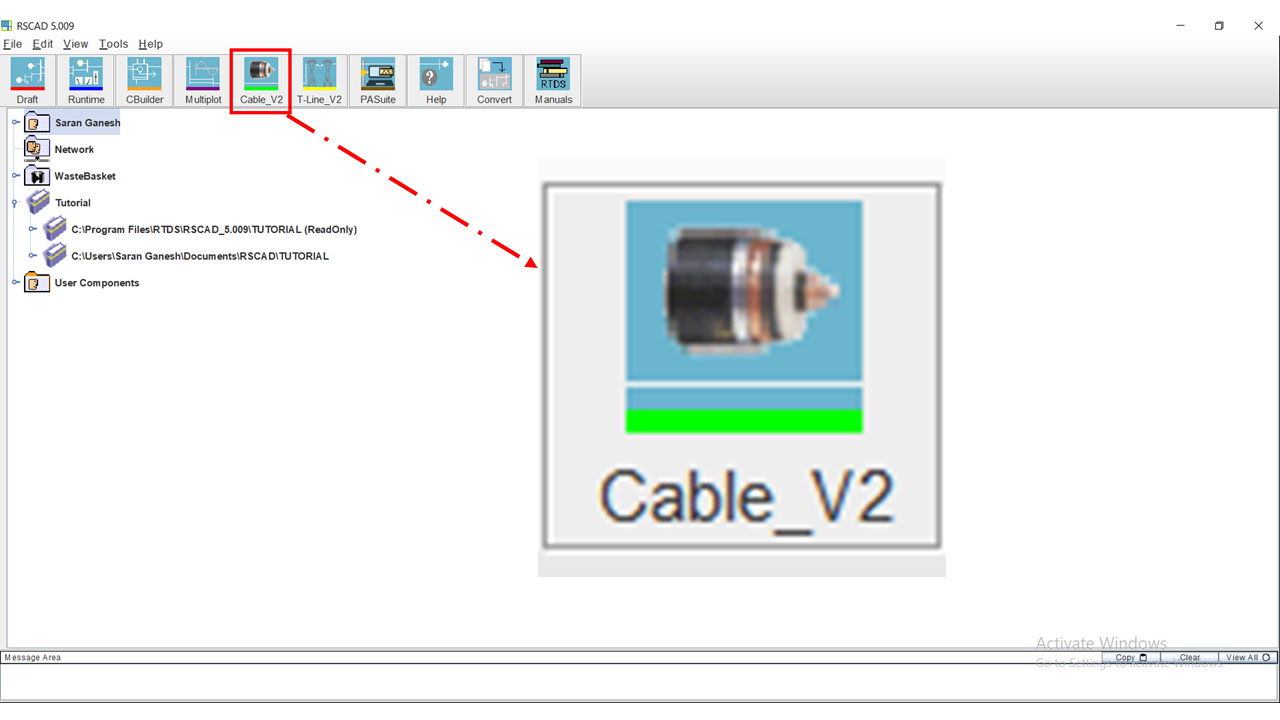
\includegraphics[height = 4.5cm,width = 7.5cm]{Diagrams/Chapter_3/Cable_module_Final.png}
    \caption{Cable module in RSCAD}
    \label{fig:CableModule_mark}
\end{figure}
%\vspace{-16mm}

\begin{figure}[H]
  \centering
  % include first image
  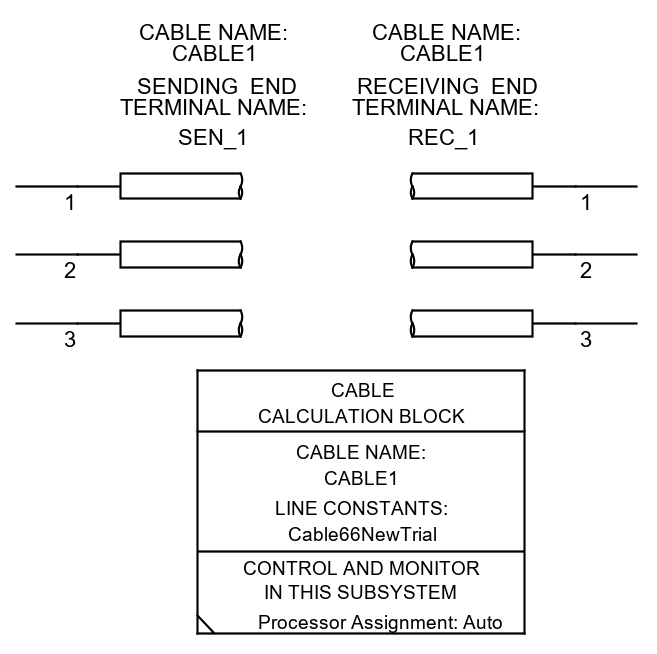
\includegraphics[height = 6cm,width = 6.5cm]{Diagrams/Chapter_3/CableParaBlock.PNG}  
  \caption{Cable configuration in Draft module in RSCAD}
  \label{fig:CableParaBlock}
\end{figure}

\subsection{External AC system}\label{ext_AC_source}
The external \gls{AC} system represents the infinite grid connection and is modelled as an \gls{AC} voltage source. The infinite grid is similar to the representation of a synchronous generator with high inertia constant. For a strong grid, typical values of inertia constant of 5 MW/MVA$^2$ depicting a synchronous generator is chosen from \cite{kothari2003modern}. The commonly represented damping constant is the frequency-dependent load damping constant. However, the damping constant is zero in this case as no loads and a lossless machine is considered. Alternatively, for short circuit calculations, the reference parameters given in \cite{wachal2014guide} can be chosen for representing a infinite grid. The parameters include short circuit power of 30 GVA and X/R \footnote{X/R = the amount of reactance X divided by the amount of resistance R} of 10. The \gls{AC} source voltage is rated at 66 kV.

\section{Control Structures}
The control strategies are implemented in the \gls{MSC} and \gls{GSC} of the Type-4 \gls{WG}. The conventional current control architecture utilized in \gls{MSC} is explained in Appendix \ref{MSC_Control}. The major area of interest for this thesis is the control strategy of \gls{GSC}. The \gls{DVC} illustrated in Section \ref{DVC_theory} is implemented in the \gls{GSC}.   

\subsection{Implementation of DVC in RSCAD}\label{DVC_RSCAD}
The control strategy depicted in \cite{korai_dynamic_2019} is achieved in RSCAD software. The control was implemented in RSCAD in \cite{sethi_real-time_nodate-new} for a 33 kV \gls{HVAC} transmission network, but the final goal of achieving reactive current injection during severe dynamic conditions was lacking. The primary reason was due to the avoidance of the current limiter block that is explained later in this section. However, the block is implemented successfully in this work, and the results are illustrated. 
Since RSCAD allows modelling of the secondary side of the transformer as required for one \gls{WG} as explained in Section \ref{scaling_OWF}, the control loop parameters of \gls{GSC} remain the same as 33 kV for a 66 kV offshore network and are based on the benchmark values provided in \cite{erlich_description_2018}. The control strategy described in Section \ref{DVC_theory} is incorporated in the reactive power and active power control loops defined in the following section. 

\subsubsection{Reactive Power Control}
From the control structure, it can be seen that, unlike in conventional current control, the reactive current is not directly utilized for voltage control. The converter voltage is directly controlled here, and this allows the current to modify on its own according to varying network conditions. This strategy is similar to the voltage control in conventional synchronous generators. The reactive control loop consists of an outer loop based on a slow VAR controller that tracks the changes in set-points required by the system-wide demand. The inner loop consists of a fast-acting controller, as the name suggests, that responds towards crucial changes in voltage where quick action is required \cite{korai_dynamic_2019}.

\begin{figure}[H]
\centering
%\hspace*{-1.2cm}
    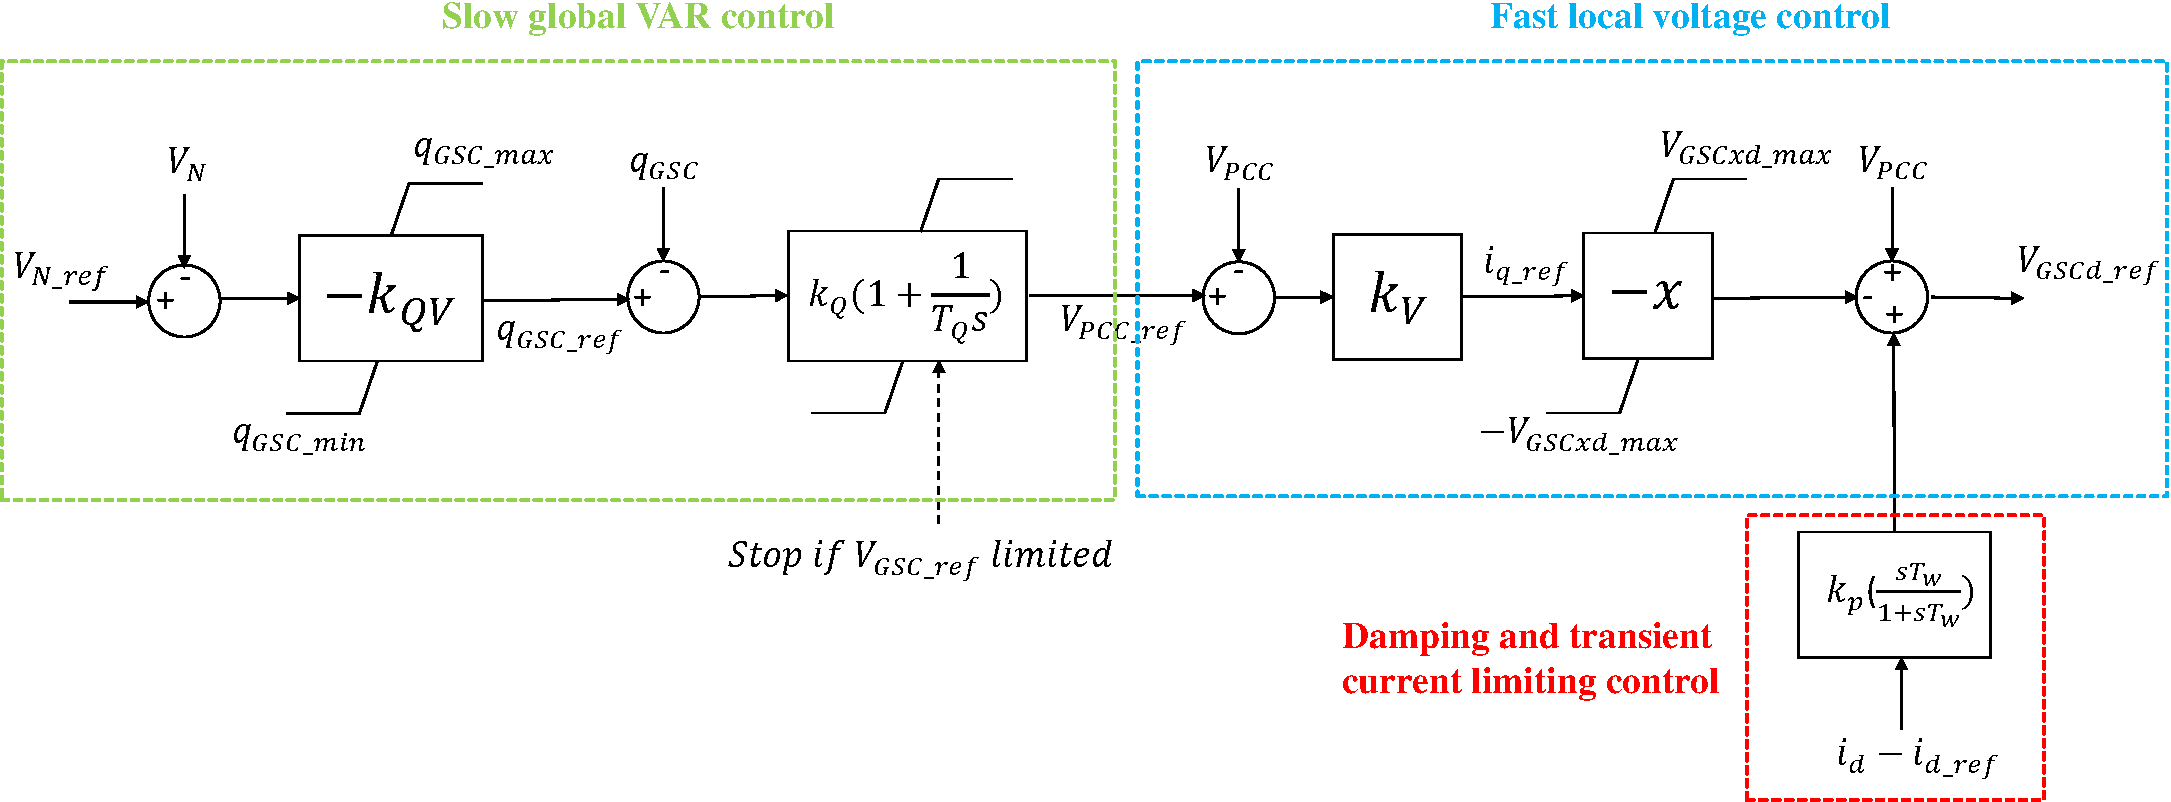
\includegraphics[height = 6.5cm,width = \textwidth]{Diagrams/Chapter_3/Reactive_power_loop.pdf}
    \caption{Reactive power control loop \cite{korai_dynamic_2019}}
    \label{fig:Reactive_Power_Control_Loop}
\end{figure}

\paragraph{Slow global VAR control}:
It is the upper-level controller and can be modelled as a power factor, reactive power or voltage controller. The reference values can be directly sent as inputs to the \gls{PI} controller if the controller is made to use for reactive power or power factor control. The voltage controller is used here, and this requires reactive power reference ($q_{GSC\_ref}$) to be determined from a predefined voltage versus reactive power droop characteristic. A voltage value for which the injection of reactive power is zero is obtained from this characteristic. The obtained reactive power reference output is provided as input to the \gls{PI} controller having a small proportional gain ($k_Q$) and ample time constant ($T_Q$) in order to avoid transformer tap changes and not very fast in order to avoid unwanted controller interactions. The automatic adjustment of reactive power in relation to varying voltage using the proportional gain, ($k_{QV}$) is significant. There is no dead-band present in order to ensure continuous voltage control. The  proportional gain that represents the droop can be obtained from the following relation,

\begin{equation}
    k_{QV} = \frac{\Delta q_{GSC}}{\Delta V_N}
\end{equation}

In theory, the proportional gain can be varied with changes in power flow. But this is not practically feasible and hence it is recommended to set the reactive power reference based on load flow calculation in the network and corresponding optimum power flow (OPF) calculations. The values could be updated at regular intervals. $V_{N\_{ref}}$ can be determined from $q_{GSC\_ref}$ as,
\begin{equation}
    V_{N\_{ref}} = -\frac{q_{GSC\_ref}}{k_{QV}} + V_N
\end{equation}
where $V_N$ is desired voltage and $V_{N\_{ref}}$ is the voltage at which no reactive power injection is required.
The reactive power limits ($q_{GSC\_max}$ and $q_{GSC\_min}$) are the continuous values in steady-state and can be computed from the P-Q diagram of the converter operation. The time constant is chosen in the range of 5-30 s wherein a value in the higher range tends to stabilize whereas a value in the lower range can cause interactions with other controllers.

The slow global VAR controller must be made inactive once the converter current limit is reached and also during cases of large voltage sags or swells by providing a signal to deactivate the controller. A scenario that could lead to the case mentioned above is a three-phase short circuit event. The output from the upper-level controller must be constant because of the chosen high integration time constant or must be limited by a blocking signal \cite{korai_dynamic_2019}.

\paragraph{Fast local voltage control}:
The voltage reference output ($V_{PCC\_ref}$) received from the slow global VAR controller is provided as input to the fast local controller. This controller must be able to provide prompt support for grid voltage during the time of faults. The response of the controller in terms of voltage support must depend on local inputs sensed at the \gls{PCC} and not on quantities that need to be measured at remote places using a communication mechanism. A proportional gain ($k_V$) is used for this purpose. The proportional gain can be obtained from the following relation \cite{korai_dynamic_2019},

\begin{equation}
    k_V = \frac{\Delta i_{Q\_GSC}}{\Delta V_N }
\end{equation}

The primary control action is provided by the feed-forward term, $x$, which is the reactance of the \gls{PE} converter (\gls{GSC}). The voltage output obtained on multiplying the current ($i_{q\_ref}$) with $x$ is the set point voltage of the converter in steady state. The reactive control loop parameters are shown in Appendix \ref{tab:Reactive_pow_para}.

\subsubsection{Active Power Control}\label{Active_power_DVC_theory}
The active power control consists of the \gls{DC} voltage, direct frequency control and Voltage Dependent Active Power Reduction (\gls{VDAPR}) control, as shown in Figure \ref{fig:Active_Power_Control_Loop}. The control of active power is provided using the q-axis component of \gls{GSC} voltage as per the Equation \ref{P_eq}. Theoretically, since the \gls{DC} capacitor provides the active power control, the \gls{DC} energy barrier should be made higher which is to be done by increasing the capacitor size and \gls{DC} voltage when in comparison with the conventional \gls{PI} based current control \cite{korai_dynamic_2019}. However, considering the practical aspect, such an increase in capacitance is not incorporated for this work and the \gls{DC} voltage is not increased and is set at 4 kV. Another significant modification that was done is providing the minimum limit, $V_{a\_lim\_min}$, for the voltage measurement. A small value needs to be set for this parameter in RSCAD software or else an error causing division by zero would be bound to occur during the start of the simulation. The active power is calculated as follows: 

\begin{equation}\label{P_eq}
    p = V_{PCC}i_d = -V_{PCC}\frac{V_{GSC\_q}}{x}
\end{equation}
%where $V_T$ is the voltage at \gls{PCC}.

The direct frequency control provides control in case of under frequency and over frequency. The control is modelled to be activated when the frequency is above 50.2 Hz or below 49.8 Hz.
The \gls{VDAPR} control is provided to control the power injection capacity of the \gls{GSC}. Since power cannot be injected to the grid by the \gls{GSC} during the time of faults, the \gls{VDAPR} allows in reducing the set point of reference power and thereby refining the dynamic stability of the network. The active control loop parameters are shown in Appendix \ref{tab:Active_pow_para}.

\begin{figure}[H]
\centering
%\hspace*{-1.2cm}
    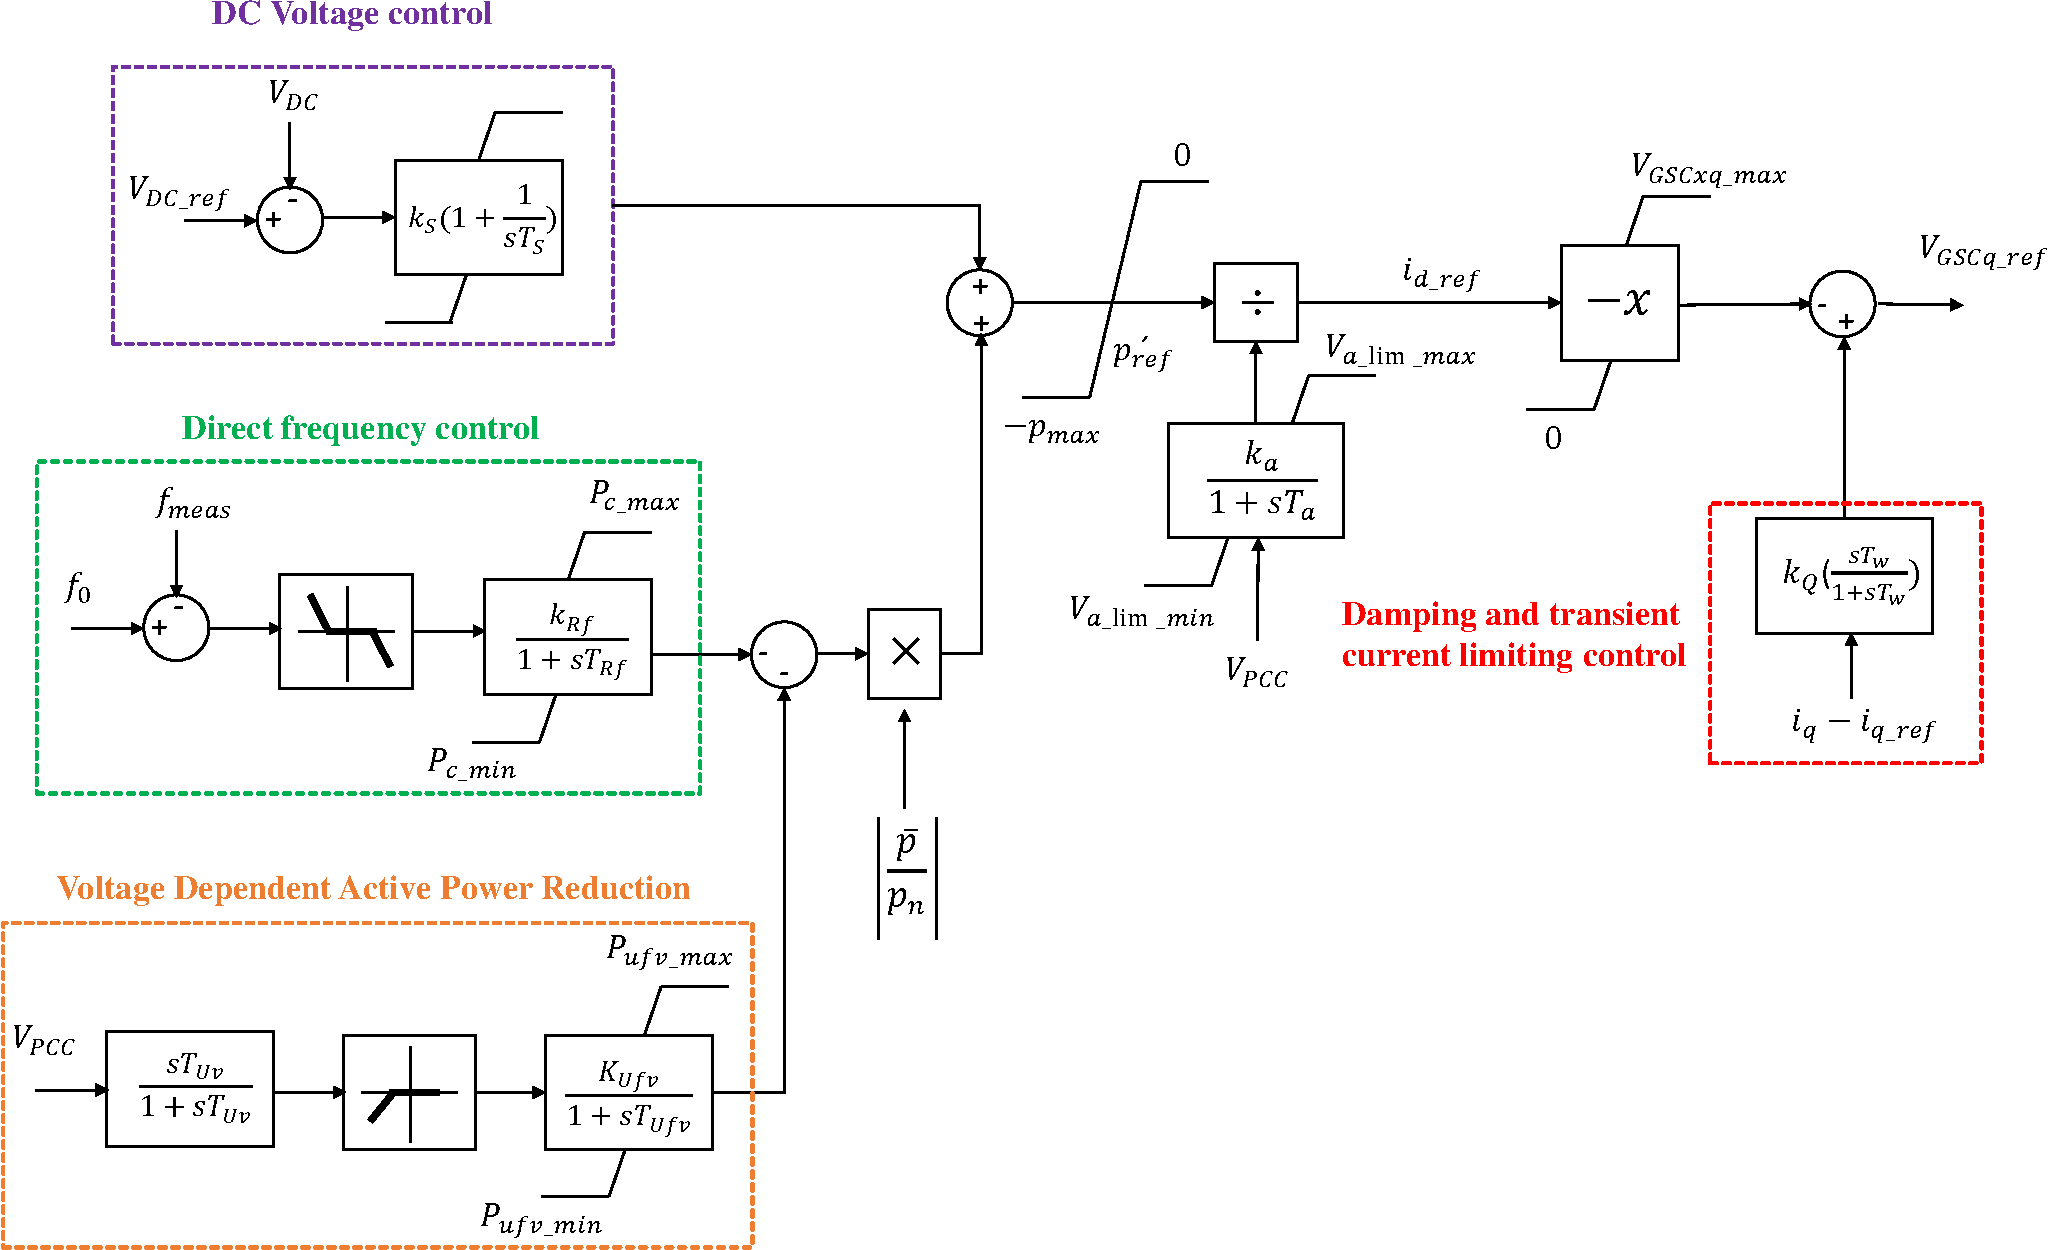
\includegraphics[height = 11cm,width = \textwidth]{Diagrams/Chapter_3/Active_power_loop.pdf}
    \caption{Active power control loop \cite{korai_dynamic_2019}}
    \label{fig:Active_Power_Control_Loop}
\end{figure}

\subsubsection{Current Limitation}\label{currentlimitation_RSCAD}
The current limitation is an important block that protects the \gls{PE} components from damage due to over current. A new maximum current ($i_{max\_ref}$) value is computed whenever the maximum current ($i_{max0\_ref}$) of the \gls{PE} converter is exceeded. The current limitation is incorporated in \gls{GSC} based on Equations \ref{currentlimeq1} and \ref{currentlimeq2}. The upper and lower limits for $i_{q\_ref}$ and $i_{d\_ref}$ are calculated based on the grid impedance (shown as Priority in Figure \ref{fig:Current_Limiter_block}) and the new maximum currents ($i_{d\_ref\_lim}$ and $i_{q\_ref\_lim}$) are computed. 
Once the reference limits are computed, the converter voltage limits are calculated by Equation \ref{vol_lim_1} or by Equations \ref{vol_lim_2} and \ref{vol_lim_3} \cite{korai_dynamic_2019}.

if
\begin{equation} \label{currentlimeq1}
% \begin{split}
  (|i_d+ji_q|-i_{max0\_ref})>0 \longrightarrow i_{max\_ref} = i_{max0\_ref} - k_{red} .(|i_d+ji_d|-i_{max0\_ref}) \\
\end{equation}

else
\begin{equation}\label{currentlimeq2}
    \\
  i_{max\_ref} = i_{max0\_ref}  
% \end{split}
 \end{equation}
 
\begin{figure}[H]
\centering
%\hspace*{-1.2cm}
    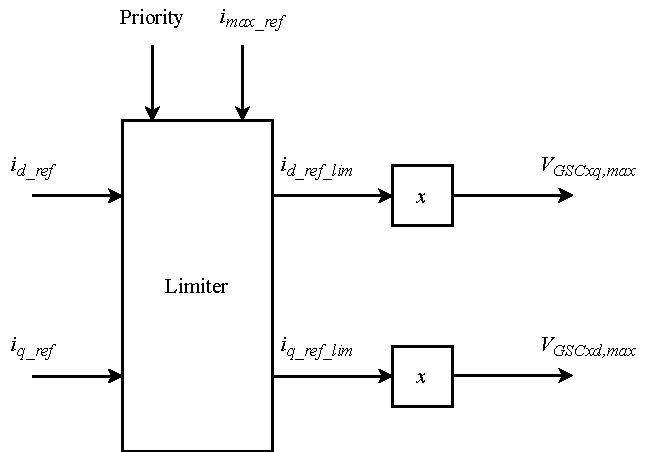
\includegraphics[height = 7.5cm,width = 10cm]{Diagrams/Chapter_3/Current_Limiter_block.pdf}
    \caption{Current limitation algorithm in VSC \cite{korai_dynamic_2019}}
    \label{fig:Current_Limiter_block}
\end{figure}

As long as the reference current is not limited,
\begin{equation}\label{vol_lim_1}
    V_{GSCxq\_max} = V_{GSCxd\_max} = x . i_{max\_ref}
\end{equation}

else

\begin{equation}\label{vol_lim_2}
    V_{GSCxq\_max} = x . i_{d\_ref\_lim} 
\end{equation}
\begin{equation}\label{vol_lim_3}
    V_{GSCxd\_max} = x . i_{q\_ref\_lim}
\end{equation}

\subsubsection{Voltage Limitation}
The \gls{AC} voltage of the \gls{GSC} is generally limited by the \gls{DC} voltage value. The factor that brings the relationship between the \gls{AC} and \gls{DC} voltages is the modulation index. The modulation index is computed, as shown in Equation \ref{MI_eq}. The maximum value of the modulation index is set around to 1, and \gls{GSC} voltage must be limited at that point to avoid non-saturation of the \gls{GSC}. 

\begin{equation}\label{MI_eq}
    m = \frac{2\sqrt{2} V_{AC}}{\sqrt{3} {V_{DC}}}
\end{equation}

\section{Analysis of the Dynamic Performance of 66 kV Test System}
After the 66 kV system is modelled, it has to be tested for operation in steady-state and dynamic conditions. The performance related to short-term voltage stability and reactive power injection by the \gls{DVC} during the most severe dynamic situation in the grid has to be analyzed. A three-phase short circuit in the middle of the \gls{HVAC} cable is chosen to test the same.

\subsection{Three-phase Line to Ground Fault}

The line to ground fault logic available in the power system library in RSCAD is adapted in this network by splitting the cable model into two halves and implementing the fault logic in the middle of the two halves as shown in Figure \ref{fig:2cablesblockwithfault}. %The fault logic is explained in Appendix \ref{fault_logic}. 
The Draft module is compiled, and after ensuring no errors, the system is run in the Runtime module. The system is stabilized with the voltage values within the tolerance limit of $\pm$ 10\% during steady-state operation.

\begin{figure}[H]
\centering
%\hspace*{-1.2cm}
    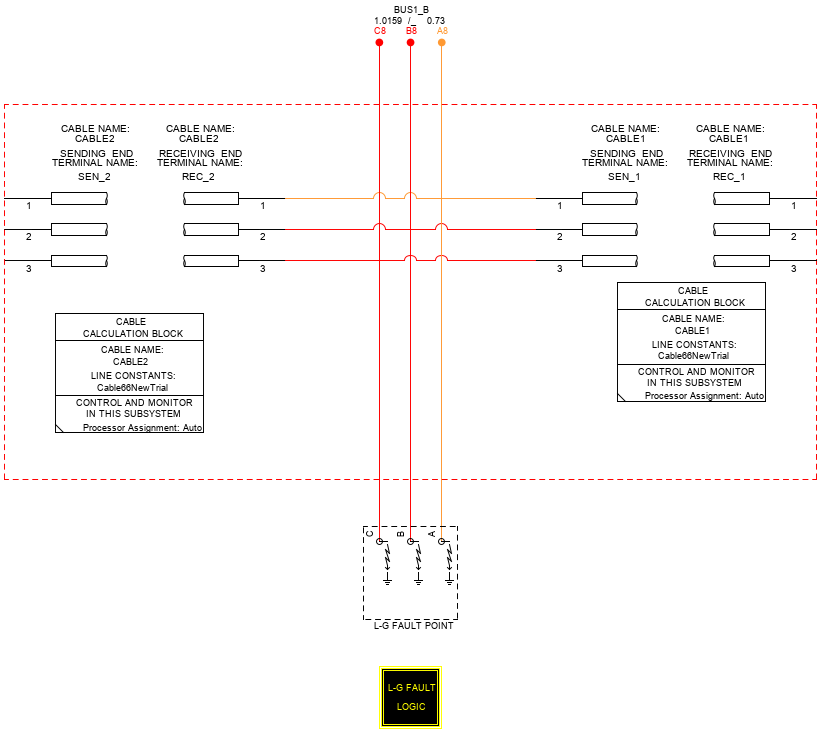
\includegraphics[height = 12.5cm,width = 13.5cm]{Diagrams/Chapter_3/2CablesBlockWithFault.png}
    \caption{Representation of three-phase fault in the middle of the cable in RSCAD}
    \label{fig:2cablesblockwithfault}
\end{figure}

The three-phase line to ground fault is applied at 0.5 s with a fault clearing time of 140 ms. The voltage and frequency responses are recorded, as shown in Figure \ref{fig:Vol_Freq_3phaseSC}. In the pre-fault condition, the voltage is stabilized at nearly 1.04 p.u., as seen in Figure \ref{fig:Vol_Freq_3phaseSC} a). 
The frequency at the \gls{PCC} computed by the \gls{PLL} is set to 50 Hz.
The \gls{OWF} is generating nearly rated active power i.e. active current of nearly 1 p.u. is provided by the \gls{GSC}, as depicted by the green line in Figure \ref{fig:ID_IQ_Final_3}. There is no reactive current or reactive power injection by the \gls{GSC} during this time as seen from the purple line in Figure \ref{fig:ID_IQ_Final_3}. 

During the time of fault, the voltage drops at \gls{PCC} as expected for a three-phase line to ground fault. There is no major drop in frequency since there are no loads connected to the \gls{OWF}. Hence the frequency control does not get activated since deviation remains within 49.8 Hz and 50.2 Hz.
\gls{DVC} allows reactive current and hence reactive power to be injected by \gls{GSC} during the time of fault to support the voltage, as shown in Figure \ref{fig:ID_IQ_Final_3}. The corresponding behaviour is a major requirement as per the grid codes during dynamic conditions, as mentioned in \cite{mohseni_review_2012}. At the same time, the active current and thus active power is limited, and hence there is no generation from the \gls{OWF} (Figure \ref{fig:ID_IQ_Final_3}). Simultaneously, the voltage across \gls{DC} link increases in order to maintain the power balance as per the Equation \ref{powbaleq}. The chopper gets activated when \gls{DC} voltage goes beyond a particular limit in order to protect the \gls{DC} link from overvoltage. After the fault is cleared, the \gls{DVC} allows for quick recovery, the voltage and powers return to the pre-fault values. 

The spikes in voltage, frequency and currents after the fault is released at 0.64 s is due to the fast dynamics of \gls{DVC}. Another important observation is the transients in the currents during the time of fault at 0.5 s in Figure \ref{fig:ID_IQ_Final_3}. These are due to the dynamic effects that arise due to the exclusion of an integrator \cite{korai_dynamic_2019}. It can be controlled by proper tuning of washout filters.

\begin{figure}[H]
%\centering
%\hspace*{-2cm}
    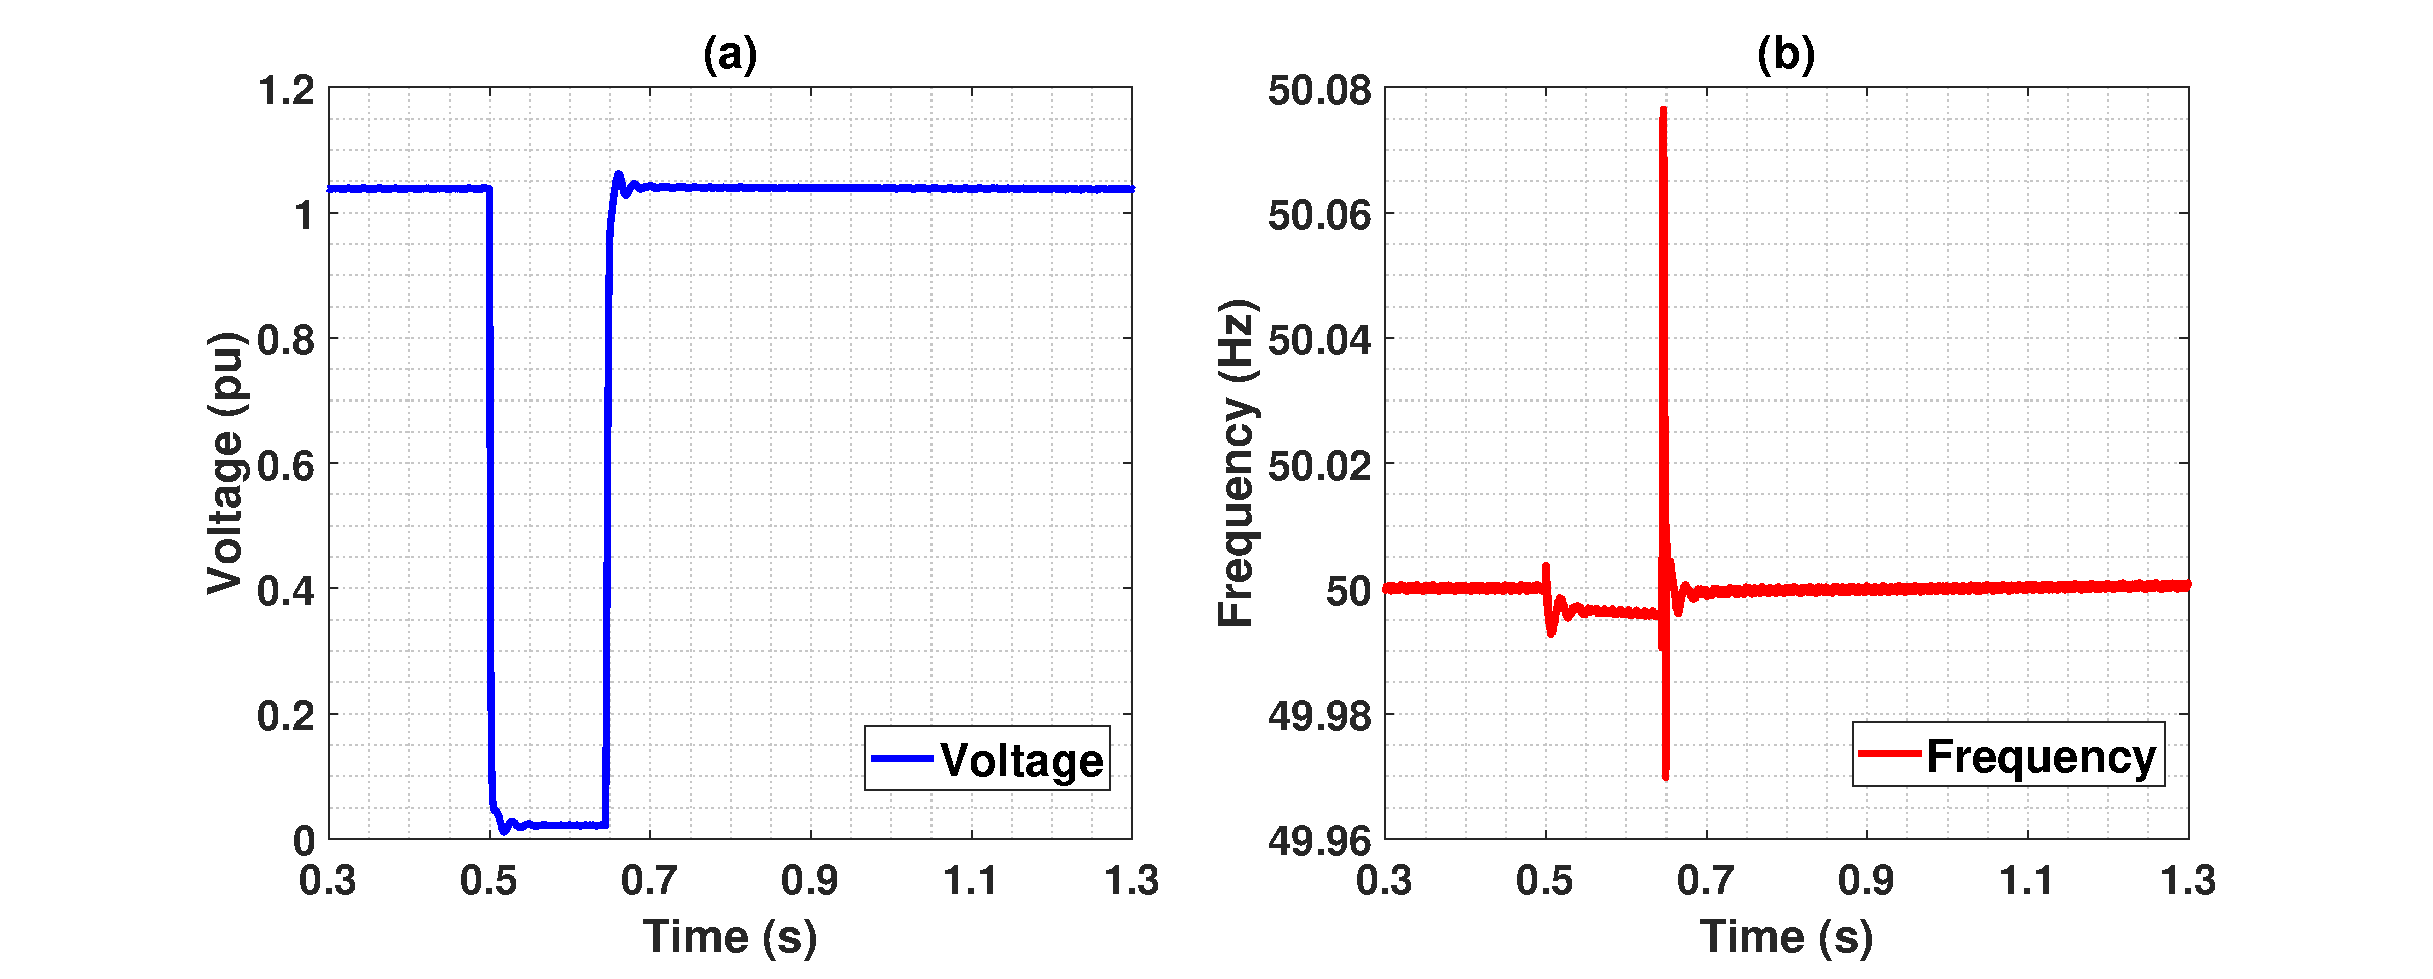
\includegraphics[height = 7cm,width = \textwidth]{Diagrams/Chapter_3/VACP_Freq_Final_3.eps}
    \caption{a) Voltage at PCC and b) Frequency response synthesised by PLL following a three phase fault in the middle of the cable}
    \label{fig:Vol_Freq_3phaseSC}
\end{figure}


\begin{figure}[H]
%\centering
%\hspace*{-0.1cm}
    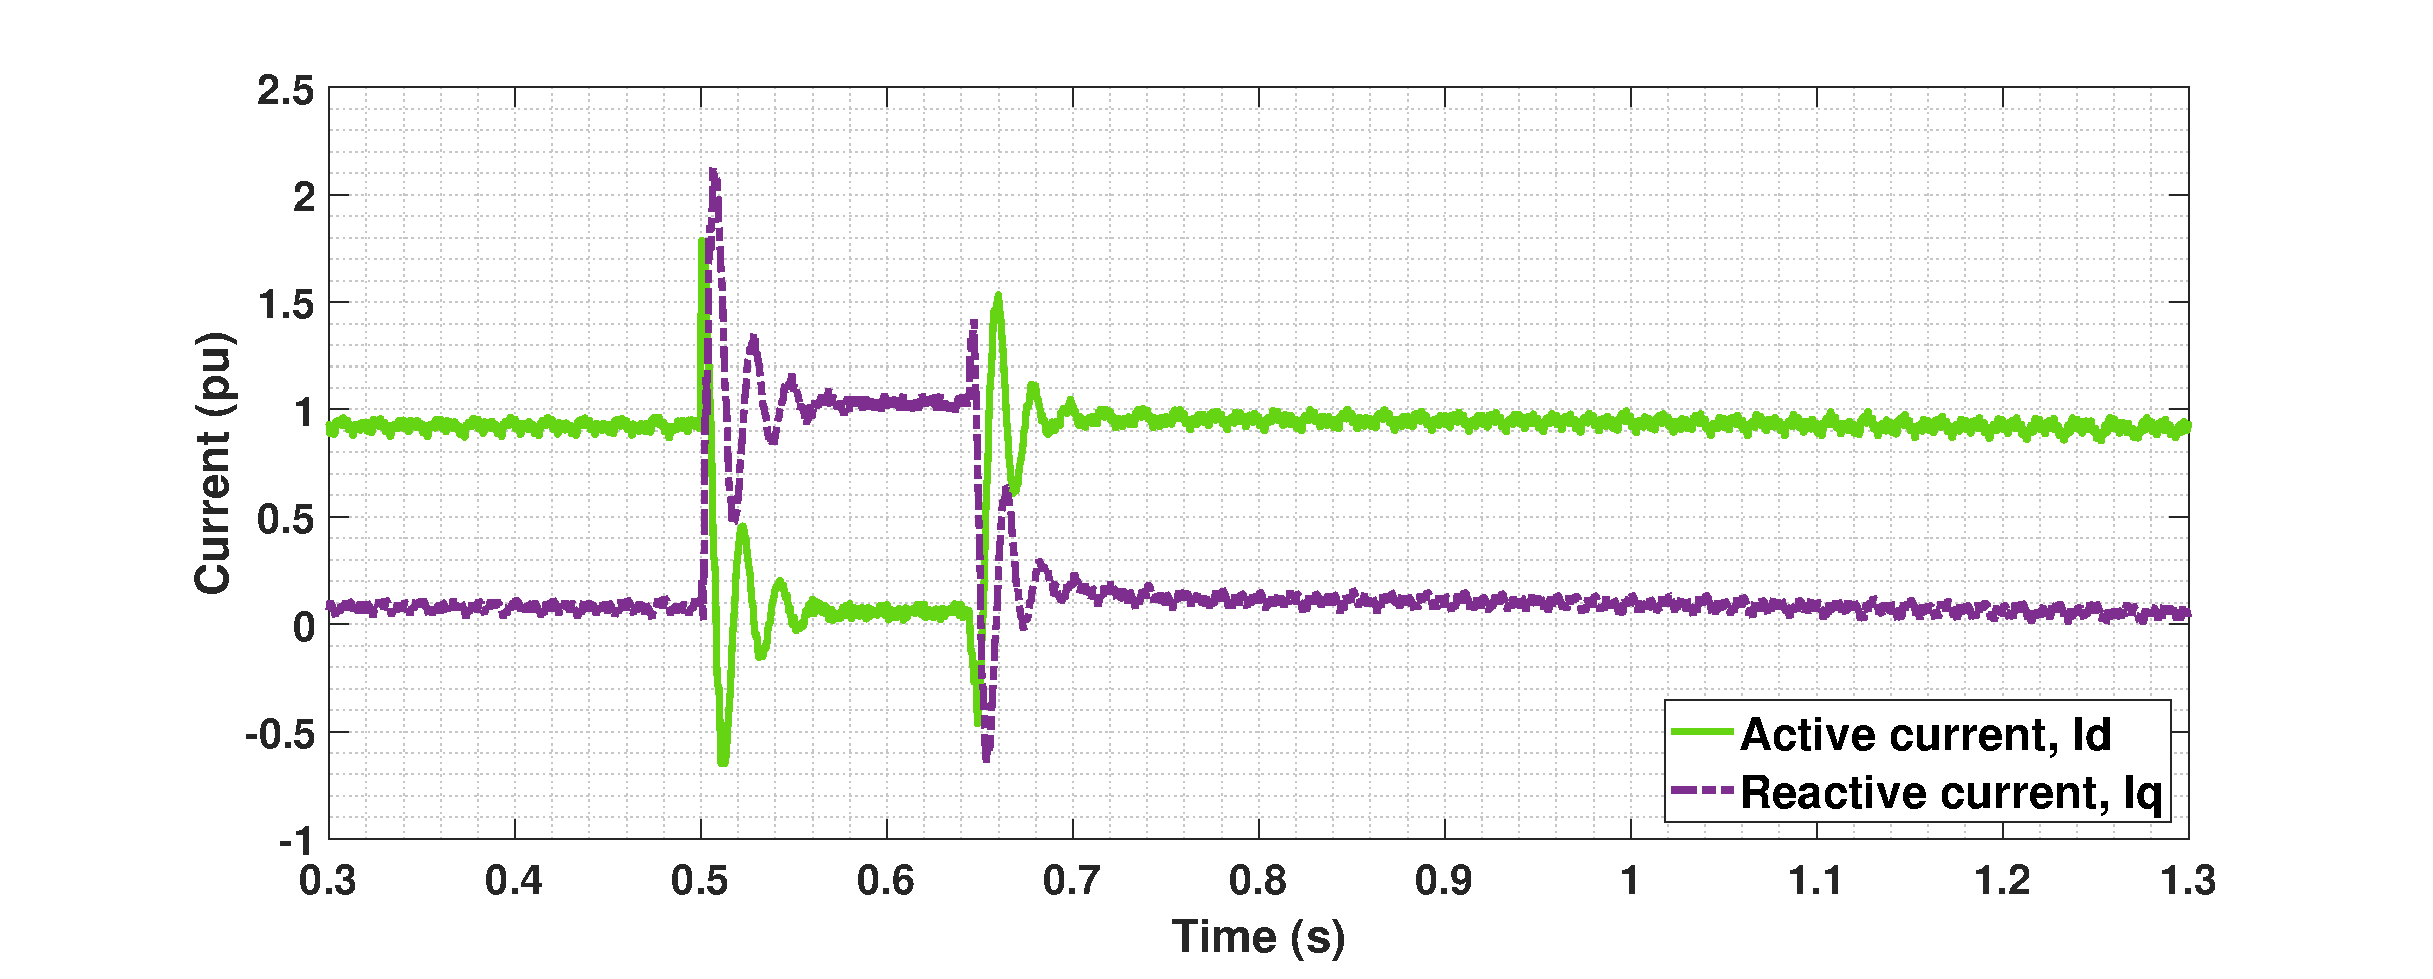
\includegraphics[height = 6.5cm,width = \textwidth]{Diagrams/Chapter_3/ID_IQ_Final_4.eps}
    \caption{Active and reactive currents flowing to the network for a three phase fault in the middle of the cable}
    \label{fig:ID_IQ_Final_3}
\end{figure}


\subsubsection{Parameter Selection for Washout Filters}\label{para_selection_washout}
The damping during the transient process mentioned in Section \ref{DVC_theory} is ensured by the washout filters in the reactive power and active power control loops as seen in Figure \ref{fig:Reactive_Power_Control_Loop} and Figure \ref{fig:Active_Power_Control_Loop} respectively. Parameter sensitivity analysis need to be performed for the washout filters to ensure fast damping of transients. The output of the washout filter for various proportional gains for a step response is depicted in Figure \ref{fig:Washout_gain_output}. The proportional gain represents values to which the output of the washout filter changes when there is a change in the input. The time constant represents the rate of this change. It can be seen that the output of the washout filter changes proportionally to the gain value specified and comes back to the initial value after a specific time, depending on the time constant mentioned.


Effect of this property of washout filter is observed in the active and reactive currents at the \gls{PCC} for a similar three-phase fault as performed in the previous section. The measurements are recorded from 0.45 s to 0.65 s in Figure \ref{fig:ID_Washout_Comp} and \ref{fig:IQ_Washout_Comp} to analyze the behaviour of the transients during the occurrence of the fault. The proportional gain is set as 0.01, 0.03 and 0.05 for comparison, keeping the time constant = 0.01 s for all the three cases. It is observed that faster damping can be achieved for higher proportional gains, as shown in Figure \ref{fig:ID_IQ_Washout_Comp}. It makes sense as the system would try to damp the transients to the maximum possible value in order to have minimum fluctuations and also to limit interactions with other controllers during this period. Thereby, it is worthy to conclude that choosing the right parameters for the washout filter is one among the key factors in this control approach.

\begin{figure}[H]
\centering
%\hspace*{-1cm}
    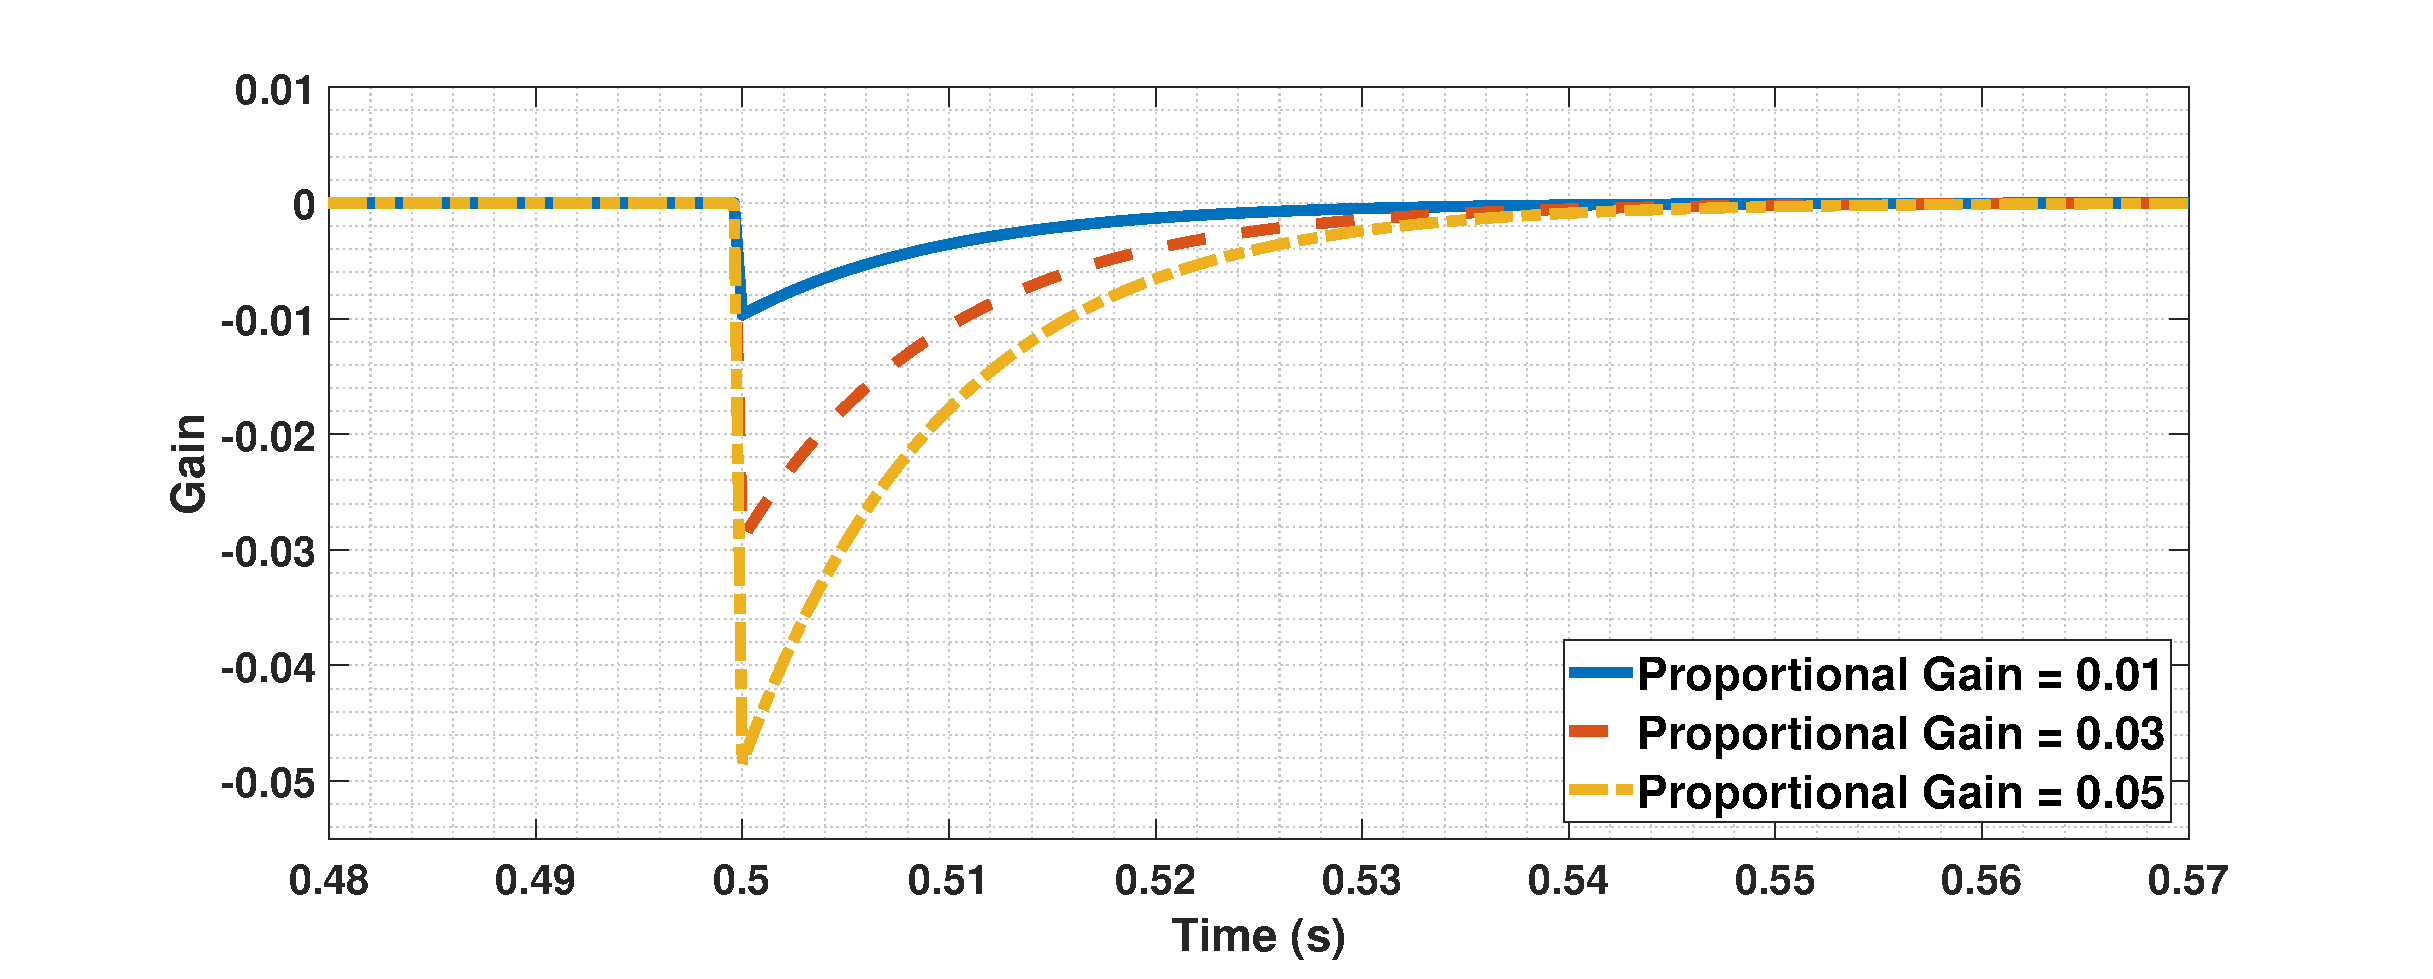
\includegraphics[height = 6cm,width = 14.5cm]{Diagrams/Chapter_3/Washout_gain_output_4.eps}
    \caption{Output of a washout filter for different proportional gains for a step response}
    \label{fig:Washout_gain_output}
\end{figure}

\begin{figure}[H]
%\centering
\begin{subfigure}{0.5\textwidth}
 % \centering
  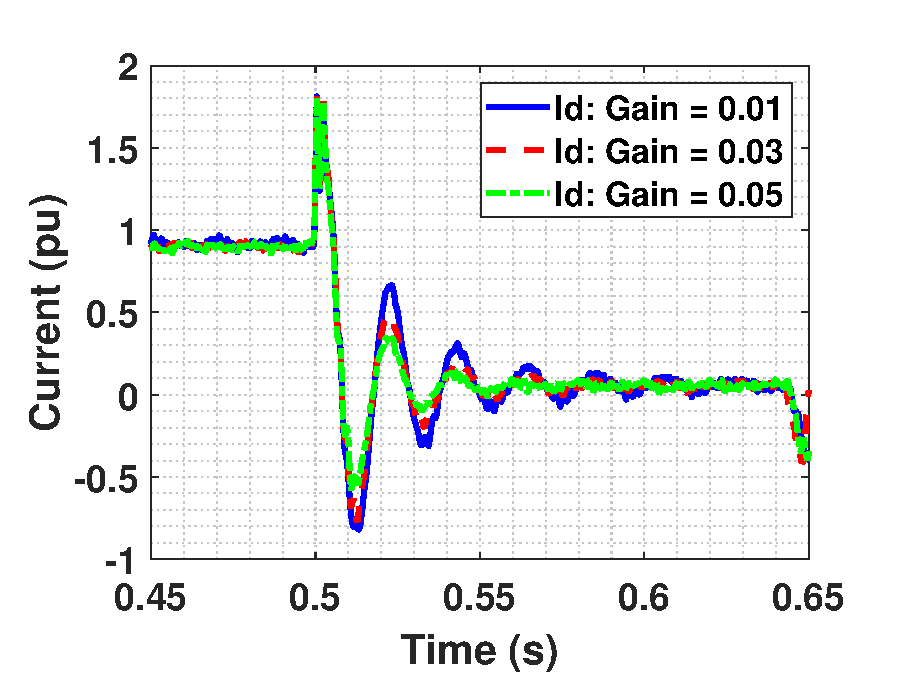
\includegraphics[height = 6.5cm,width = \textwidth]{Diagrams/Chapter_3/ID_Washout_Comp_4.eps}
  \caption{Current in d axis during three phase fault for gain 0.01, 0.03 and 0.05}
  \label{fig:ID_Washout_Comp}
\end{subfigure}%
\begin{subfigure}{0.5\textwidth}
  %\centering
  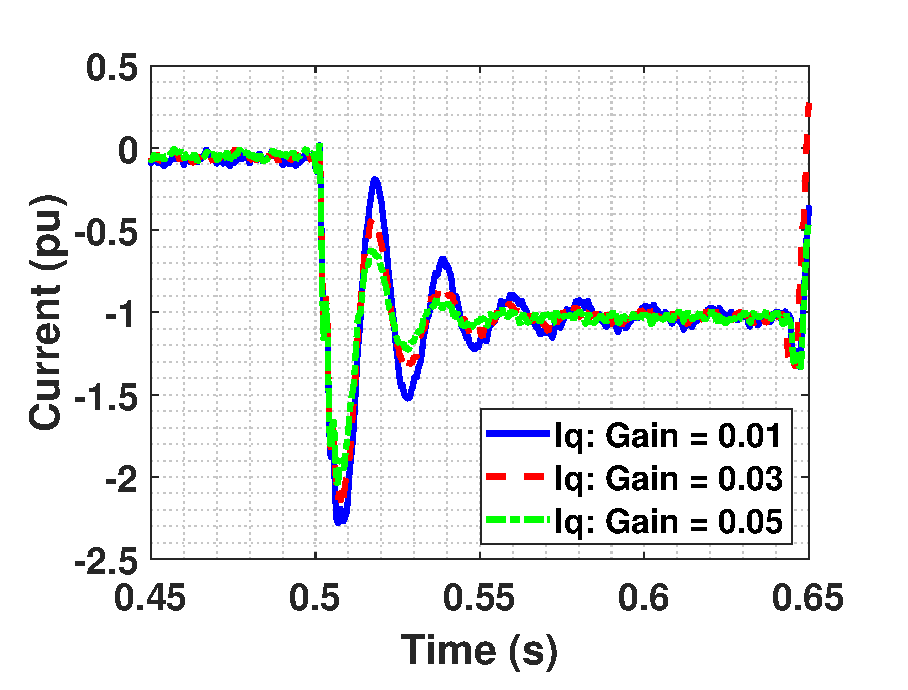
\includegraphics[height = 6.5cm,width = \textwidth]{Diagrams/Chapter_3/IQ_Washout_Comp_4.eps}
  \caption{Current in q axis during three phase fault for gain 0.01, 0.03 and 0.05}
  \label{fig:IQ_Washout_Comp}
\end{subfigure}
\caption{Currents in d and q axes during three-phase fault in the middle of the cable for different proportional gains of washout filters}
\label{fig:ID_IQ_Washout_Comp}
\end{figure}

\section{DIgSILENT PowerFactory Software}
PowerFactory is a software tool developed by DIgSILENT (Germany) that is used for RMS and EMT simulations. It has three integration characteristics; functional integration, vertical integration and database integration. Functional integration explains that PowerFactory is a single executable program and vertical integration means that the models in the power system can exchange all of the analysis functions at one place. PowerFactory uses a Data Manager for database integration that allows all models to be stored under one project file. There are two libraries available in PowerFactory; Global and Project libraries. There are two subsections available within the Project library. They are \cite{powerfactory_tech}:
\begin{itemize}
    \item Equipment Type Library
    \item User Defined Models
\end{itemize}
PowerFactory also provides development of user-defined models using DIgSILENT Simulation Language (DSL). These features are utilized, and \gls{DVC} control is implemented in PowerFactory for a typical configuration of the offshore network in \cite{korai_dynamic_2019}. It is tested and proved to work \cite{korai_dynamic_2019}. The test results achieved in RSCAD in the previous section need to be compared with a similar 66 kV \gls{HVAC} offshore network in PowerFactory to validate the control action. In this section, a 66 kV \gls{HVAC} offshore network is developed in PowerFactory with the benchmark \gls{DVC} model utilized from \cite{korai_dynamic_2019}. Differences in the models are notified, the voltage and current profiles are compared for a three-phase line to ground fault in the middle of the cable.

\section{Layout of the 66 kV HVAC Test System in PowerFactory}

The 66 kV offshore network is modelled in PowerFactory as shown in Figure \ref{fig:WT1_Model_PFD_comp}. The network consists of the following components:

\begin{itemize}
    \item A simplified model of Full Scale Converter (\gls{FSC}) based Type-4 \gls{WG} system consisting of the following elements:
    \begin{itemize}
        \item \gls{DC} circuit
        \item Grid Side Converter (\gls{GSC}) or Line Side Converter (\gls{LSC})
    \end{itemize}
    \item High Pass filter (\gls{HPF}) with series reactor
    \item \gls{OWF} transformer
    \item \gls{HVAC} cables  
    \item External \gls{AC} system
\end{itemize}

\begin{figure}[H]
%\centering
%\hspace*{-1.2cm}
    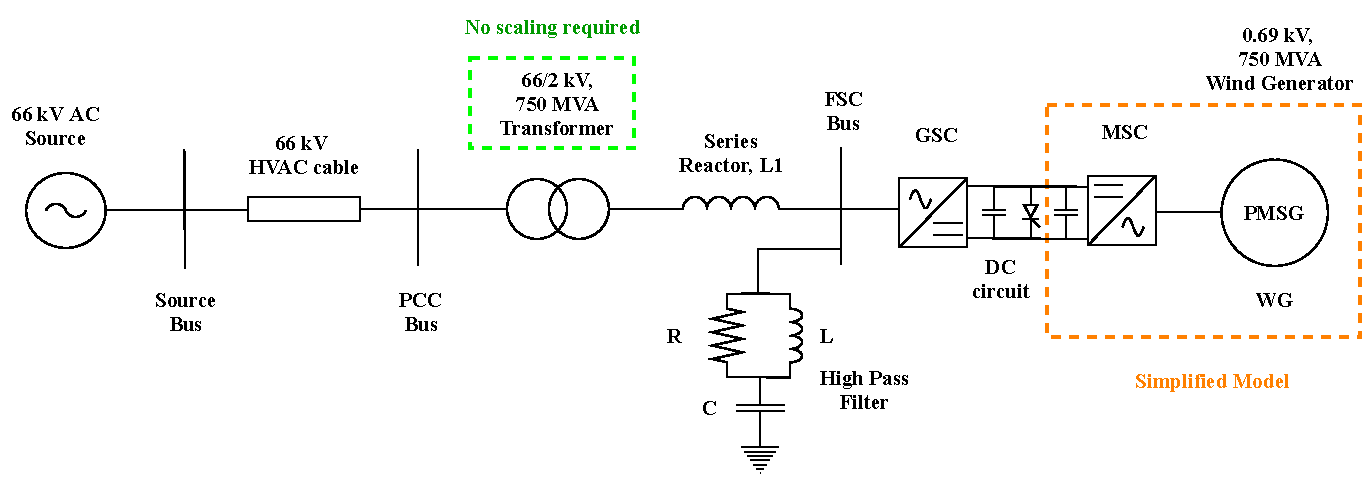
\includegraphics[height = 6cm,width = \textwidth]{Diagrams/Chapter_3/WT1_AC_PFD.pdf}
    \caption{Single line diagram of the 66 kV HVAC offshore test network in PowerFactory}
    \label{fig:WT1_Model_PFD_comp}
\end{figure}

\subsection{Simplified FSC based WG System}\label{simplified_FSC_WG}
The wind turbine and \gls{MSC} are simplified since they do not contribute to the dynamics of grid. \gls{LSC} is modelled in detail. A constant injection of active current is proposed from the \gls{MSC} to the \gls{DC} side \cite{korai_dynamic_2019}. Hence it is modelled as a \gls{DC} current source. The \gls{WG} unit is represented as a static generator model with 750 MVA nominal apparent power. It is made to operate with constant reactive power (Q) control in order to achieve the active and reactive power set points same as in RSCAD model. The active power flow is set to 700 MW, similar to the RSCAD model.

\subsubsection{DC Circuit}
The DC circuit is detailed and the voltage across the capacitor is set to 4 kV, same as the RSCAD model. The chopper activation control is provided when the \gls{DC} voltage crosses a minimum set value. 

\subsubsection{Grid Side Converter (GSC)}
Unlike the RSCAD model, a two-level \gls{GSC} is utilized in this model. The \gls{PWM} is not used in this model, and the \gls{GSC} is modelled as a controlled voltage source. This is one among the major difference with the RSCAD model. The \gls{DVC} control for \gls{GSC} developed in \cite{korai_dynamic_2019} is provided in this model as explained in Section \ref{DVC_RSCAD}. The full representation of \gls{DVC} with active and reactive power loops in PowerFactory is depicted in Appendix \ref{pfd_model_appen}. 

\subsection{High Pass Filter (HPF) with Series Reactor}
The shunt filter available in the PowerFactory drawing toolbar is chosen. The values for R, L and C are chosen the same as mentioned in Section \ref{HPF_design}. A common impedance element available in the drawing tool is chosen for the series reactor and is connected at the output of \gls{LSC}, as shown in Figure \ref{fig:WT1_Model_PFD_comp}. The inductance value chosen is the same as the RSCAD model to have an equal impedance for both the models.  

\subsection{OWF Transformer}
A two winding transformer available in the equipment library folder of DIgSILENT library is used. The transformer is rated 66/2 kV, 750 MVA with a wye-delta configuration to block zero sequence currents. The leakage inductance and resistance of the transformer are set the same as the RSCAD model.

\subsection{HVAC Cables}
The cables are rated at 66 kV same as the RSCAD model. The cable is modelled from the "Cables" section available in the equipment library in DIgSILENT library. The type of model is chosen to be the Pi model. %as shown in Figure \ref{fig:CableModel_PFD}. 
Pi model is utilized as it is easier to input the cable parameters in terms of RLC in both RSCAD and PowerFactory.

\subsection{External AC system}
The external \gls{AC} system in PowerFactory also represents an infinite grid. Similar to the model in RSCAD in Section \ref{ext_AC_source}, the infinite grid is modelled as a \gls{AC} voltage source available in the PowerFactory drawing toolbar. 

\section{Control Structures}
As mentioned in Section \ref{simplified_FSC_WG}, the wind turbine and \gls{MSC} models utilized are simplified and is made to inject constant active current to the \gls{DC} circuit. Hence, the control of \gls{MSC} and wind turbine is not required to be modelled. However, control structures are detailed for the \gls{DC} circuit and the \gls{GSC}. The benchmark model of \gls{DVC} from \cite{erlich_description_2018} is utilized here for the \gls{GSC}. The control structures are depicted in Appendix \ref{pfd_model_appen}.      

\section{Comparison of Models in RSCAD and PowerFactory }
The major differences between the 66 kV \gls{HVAC} network built in RSCAD and PowerFactory are illustrated in Table \ref{tab:Comp_RSCAD_PFD_Para}. 
\vspace{-1mm}
\begingroup
%\setlength{\tabcolsep}{10pt} % Default value: 6pt
\renewcommand{\arraystretch}{1.2} % Default value: 1
\begin{table}[H]
\centering
%\hspace*{-0.5cm}
\begin{tabular}{|c|c|c|}
\hline
\textbf{Parameters}   & \textbf{RSCAD}         & \textbf{PowerFactory}             \\ \hline
WG model      & PMSG   & Simplified (Constant power model)                                \\ \hline
MSC control   & Conventional current control     & Not modelled           \\ \hline
GSC model & {VSC with PWM} & \multicolumn{1}{l|}{Controlled Voltage Source with no PWM}  \\ \hline
Generated active power from WG  & 6 MW  & 700 MW                                    \\ \hline
Scaling factor at transformer & 117 (cf. Section. \ref{scaling_OWF}) & Not applicable                           \\ \hline
\end{tabular}
\caption{Differences in models in RSCAD and PowerFactory}
\label{tab:Comp_RSCAD_PFD_Para}
\end{table}
\endgroup

%\vspace{-6mm}
\textbf{Representation of \gls{GSC}}: One of the differences in both models is the usage of average model representation of \gls{VSC} with \gls{PWM} in RSCAD for the \gls{GSC}, whereas a controlled voltage source model is utilized in the PowerFactory model.
\vspace{3mm}

\textbf{Scaling of power}: Another significant difference between the two models is that the components connected to the secondary side of the transformer are modelled for one \gls{WG} of 6 MW in RSCAD whereas it is directly modelled for 700 MW in PowerFactory. The scaling of power to 700 MW in RSCAD is done at the 66/2 kV \gls{OWF} transformer, as explained in Section \ref{scaling_OWF}. This helps in modelling and analysis in the real world in terms of single \gls{WG}.
\vspace{-3mm}
\paragraph{}
However, it must be noted that these differences does not affect the performance of the control operation and both the models have equal immpedances that makes the comparison significant. 

\subsection{Selection of Time Step in RSCAD and PowerFactory}
Before the start of the simulation, a specific time step value suitable for both the RSCAD and PowerFactory models need to be set. As mentioned in Section \ref{OWF}, the ratio of large time step to small time step needs to higher than 12 in RSCAD model if NovaCor processor is used. Since the small time step is chosen to be 2500 ns for the RSCAD model as mentioned in Section \ref{OWF}, a value of 50 $\mu$s is chosen for the large time step. The setting can be done by right-clicking on the Draft module and selecting "Circuit Options" in RSCAD. In PowerFactory, it can be edited in the "Step Size" option available in the "Calculation of initial conditions" tab, as shown in Figure \ref{fig:Stepsize_RSCAD_PFD}.  

\begin{figure}[H]
\centering
%\hspace*{-1.2cm}
\begin{subfigure}{.55\textwidth}
  \centering
  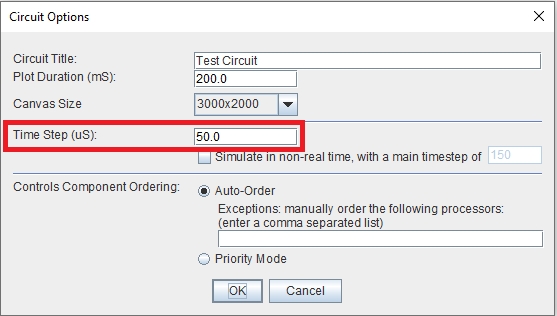
\includegraphics[height=4cm,width=7.2cm]{Diagrams/Chapter_3/Stepsize_RSCAD.PNG}
  \caption{Time step setting in RSCAD}
  \label{Stepsize_RSCAD}
\end{subfigure}%
\begin{subfigure}{.45\textwidth}
  \centering
  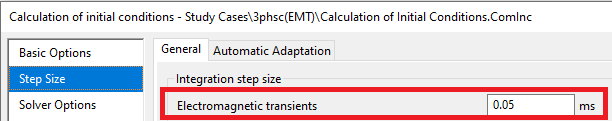
\includegraphics[height=1.6cm,width=7cm]{Diagrams/Chapter_3/Stepsize_PFD_Zoom.PNG}
  \caption{Time step setting in PowerFactory}
  \label{Stepsize_PFD_Zoom}
\end{subfigure}
\caption{Initialization of time step in RSCAD and PowerFactory}
\label{fig:Stepsize_RSCAD_PFD}
\end{figure}

\subsection{Event Comparison in RSCAD and PowerFactory}
The 66 kV offshore network model in RSCAD and PowerFactory are compared for a three-phase short circuit in the middle of the cable. A fault is applied at 0.5 seconds with a clearing time of 140 ms. The resulting voltage and current waveforms are as shown in Figure \ref{fig:VACP_comp},  \ref{fig:ID_fullACSource} and \ref{fig:IQ_fullACSource} respectively. As can be observed in Figure \ref{fig:VACP_comp}, voltage measured at \gls{PCC} drops and the generation is stopped during the fault period. The voltage profile is the same in RSCAD and PowerFactory models during the pre-fault, fault and post fault conditions as can be observed. The drop in voltage in both the graphs is the same due to equal impedance in both the models. 

\begin{figure}[H]
%\centering
%\hspace*{-1.2cm}
    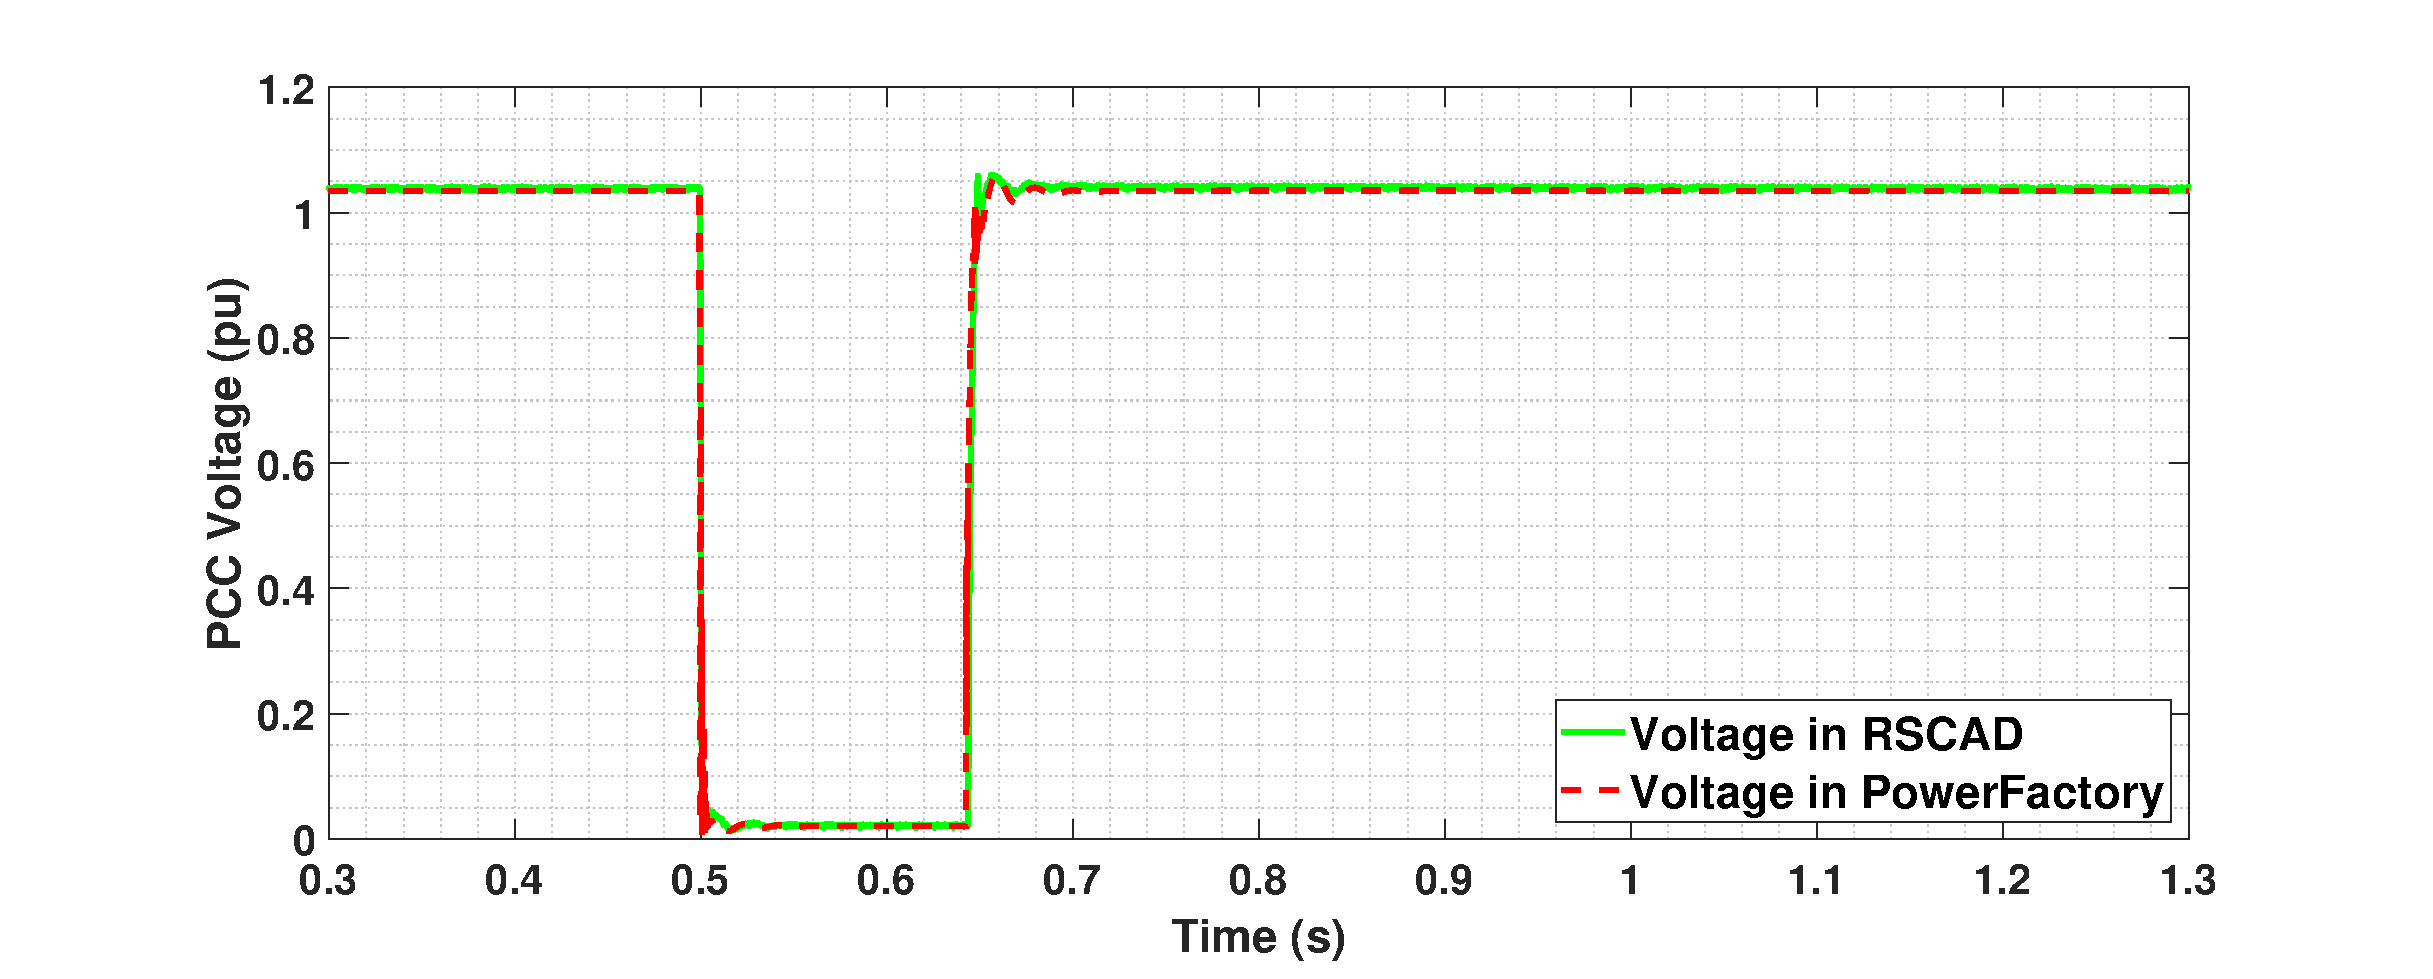
\includegraphics[height = 6.5cm,width = \textwidth]{Diagrams/Chapter_3/VACP_Comp_New_4.eps}
    \caption{Voltage measured at PCC for a three phase fault in the middle of the cable in RSCAD and PowerFactory}
    \label{fig:VACP_comp}
\end{figure}

Due to the unavoidable modelling differences in the software packages, the currents are measured at \gls{PCC} bus for the RSCAD model and at \gls{FSC} bus for the PowerFactory model. However, this does not affect the magnitude as the currents are measured in per unit. The currents in both the models have a similar profile, as summarized for the d-axis in Figure \ref{fig:ID_fullACSource} and q-axis in Figure \ref{fig:IQ_fullACSource}. The active and reactive currents generated by the \gls{WG} have the same set points in both the models during the pre-fault condition confirming that the power flow in both the models is similar. As the parameters for \gls{DVC} are the same for both the models, the reactive power injection in RSCAD model during the time of fault is achieved similar to the PowerFactory model. The transients occurring during the time of fault at 0.5 s can be damped by controlling the parameters of the washout filters, as seen in Section \ref{para_selection_washout}. The spike in the profiles at the time of fault clearance at 0.64 s is due to the fast dynamics of the \gls{PLL} in both the software packages. It is observed that the currents in RSCAD model have slight transients throughout the simulation. This is due to the detailed model representation of the \gls{GSC} in RSCAD when compared to a simplified representation in PowerFactory. Therefore, it can be concluded that the RSCAD model with the implemented \gls{DVC} provides similar results as the benchmark PowerFactory model. Moreover, the results from RSCAD model are more detailed and hence can be used as a base model for reference as it provides a better representation of the real-world operation.  


% \begin{figure}[H]
% %\centering
% %\hspace*{-1.2cm}
%     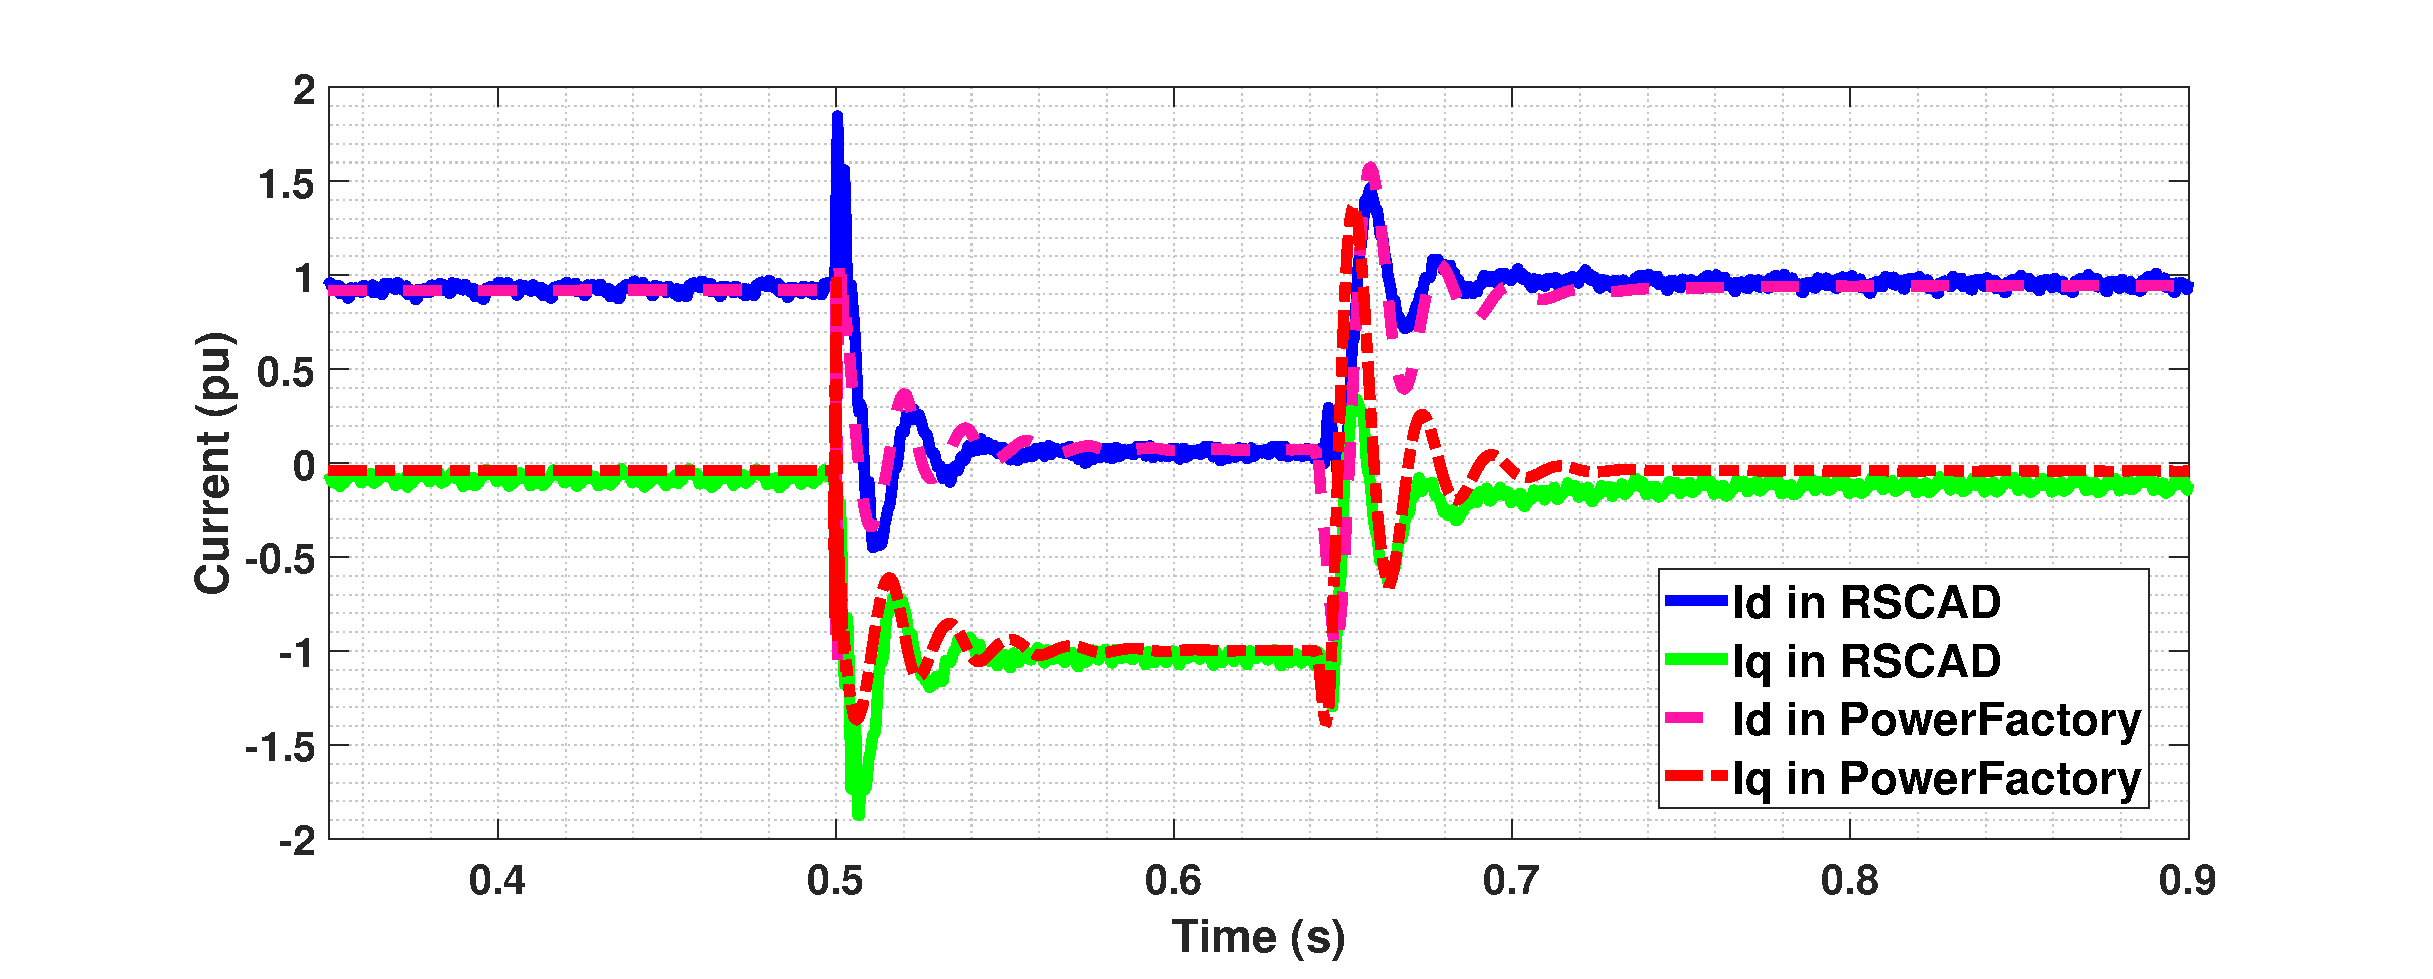
\includegraphics[height = 6cm,width = \textwidth]{Diagrams/Chapter_3/ID_IQ_Comp_New_3.eps}
%     \caption{Active and reactive currents measured for a three phase fault in the middle of the cable in RSCAD and PowerFactory}
%     \label{fig:ID_IQ_Comp}
% \end{figure}


\begin{figure}[H]
%\centering
%\hspace*{-0.1cm}
    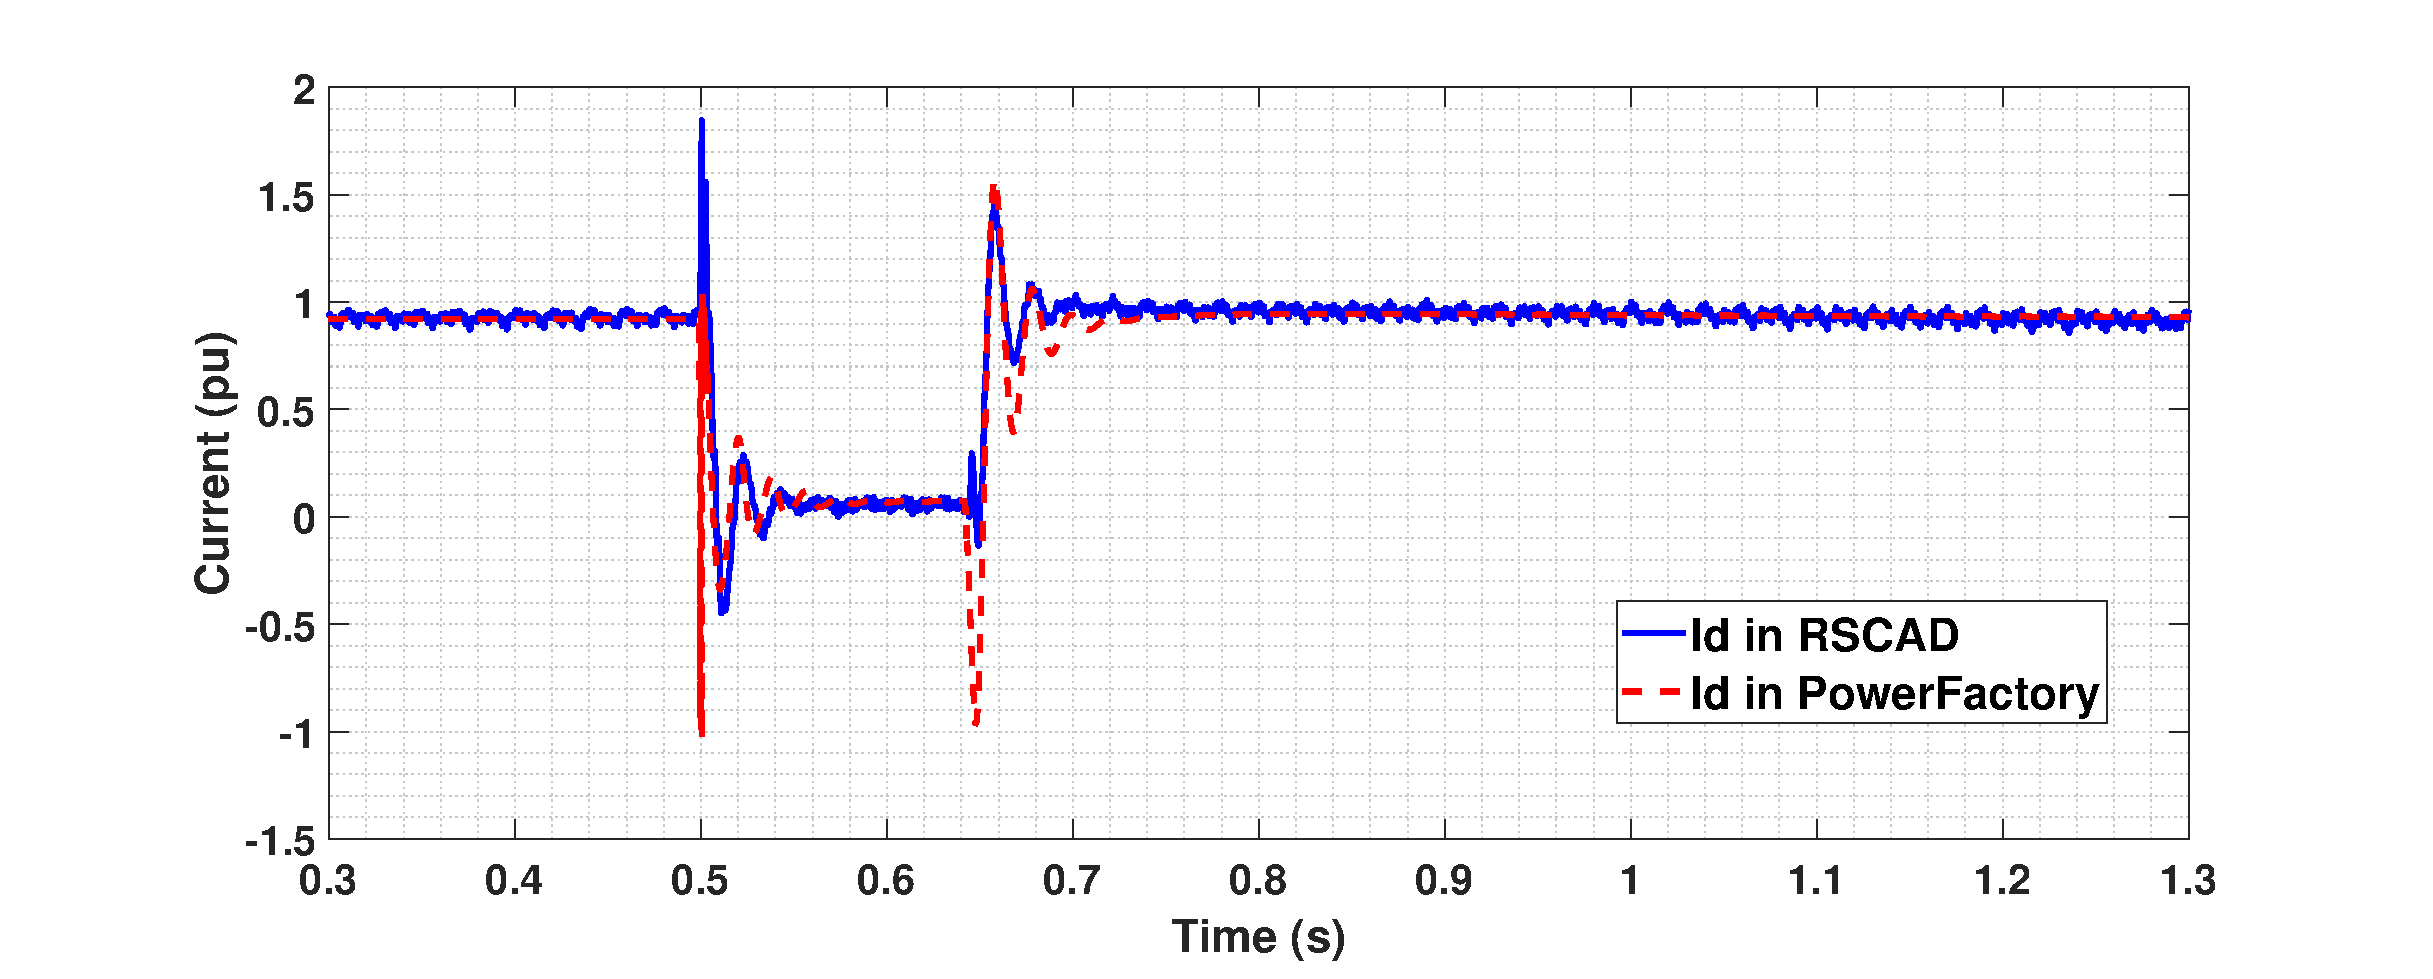
\includegraphics[height = 6.5cm,width = \textwidth]{Diagrams/Chapter_3/ID_RSCAD_PFD_Comp.eps}
    \caption{Active currents flowing to the network for a three phase fault in the middle of the cable}
    \label{fig:ID_fullACSource}
\end{figure}
%\vspace{-10mm}
\begin{figure}[H]
%\centering
%\hspace*{-0.1cm}
    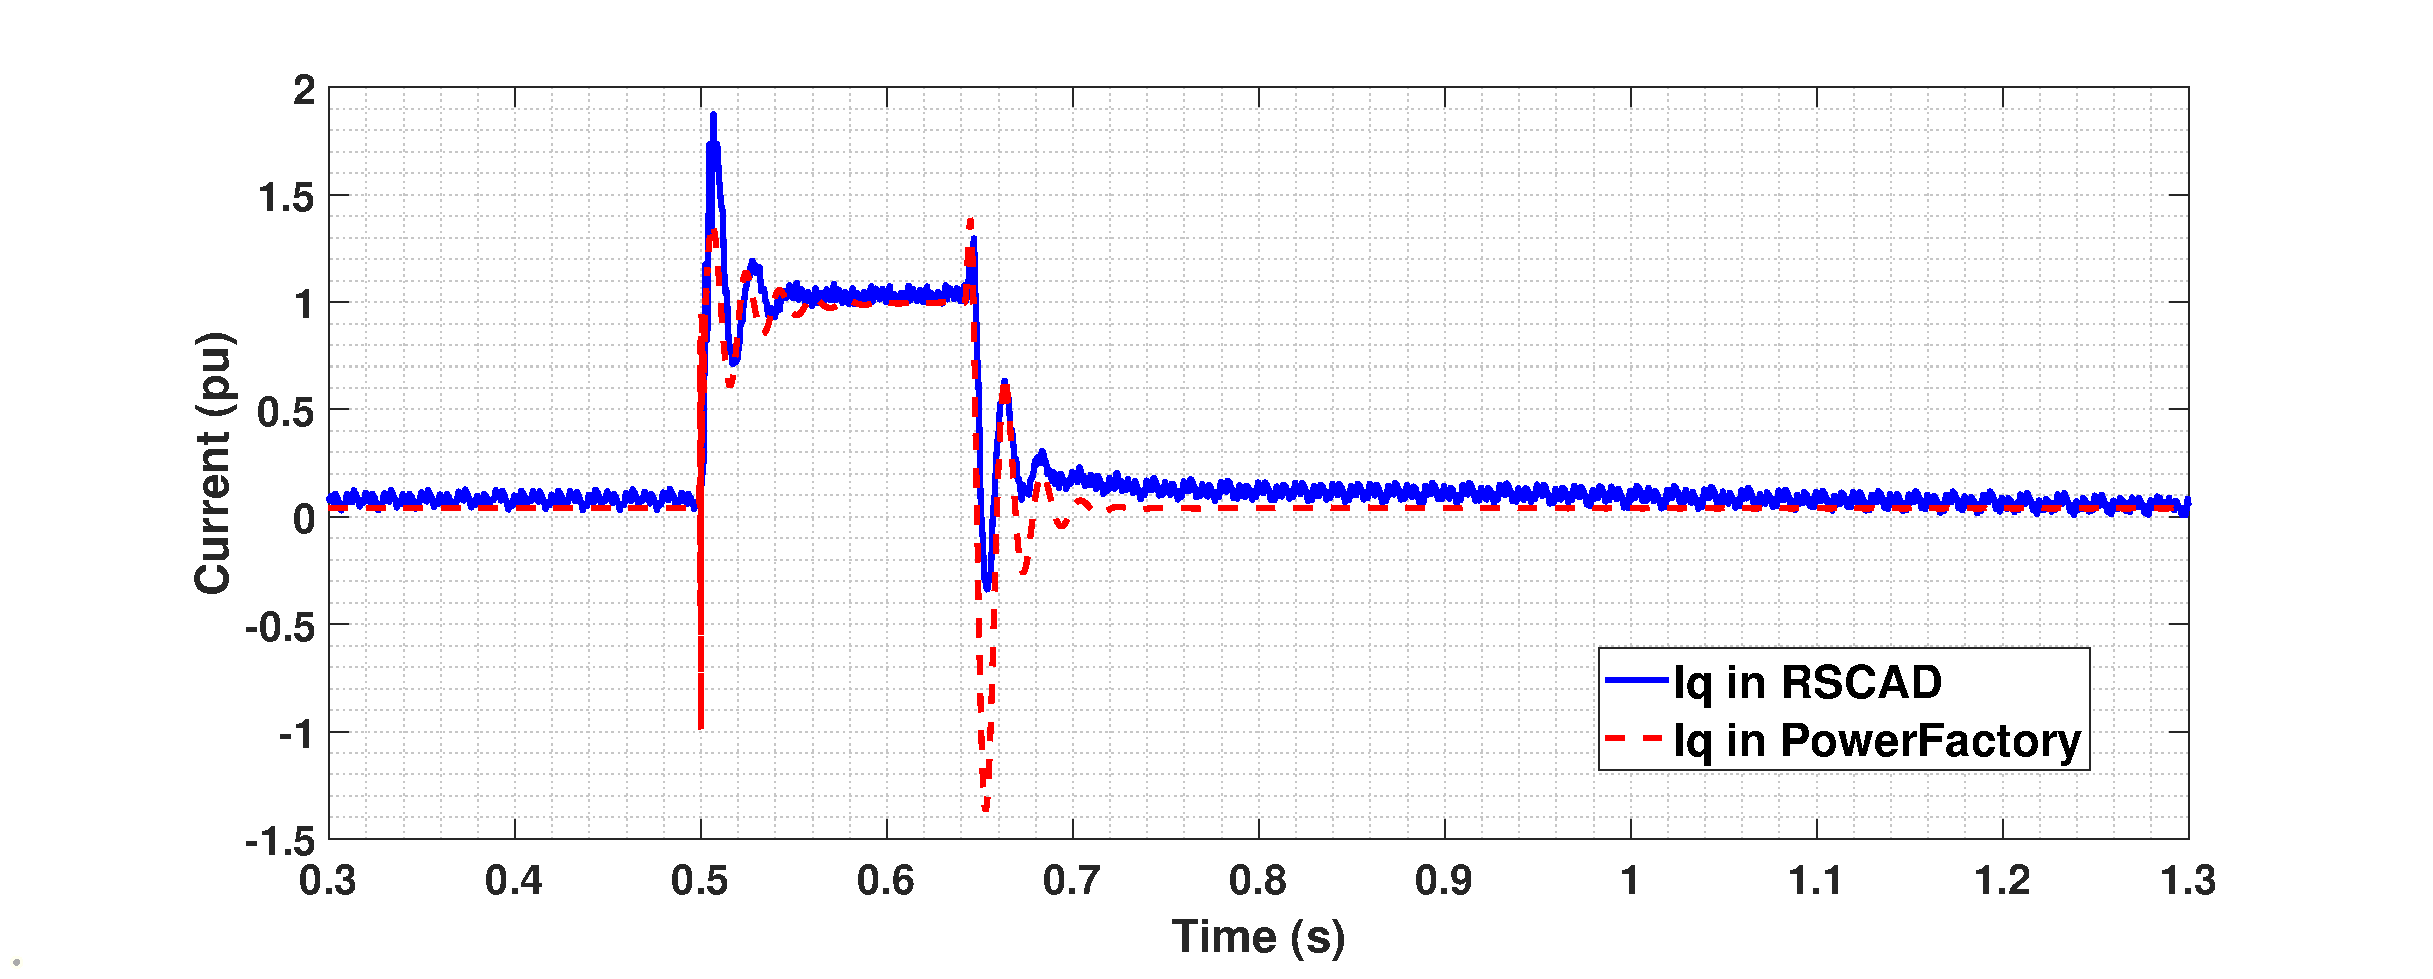
\includegraphics[height = 6.5cm,width = \textwidth]{Diagrams/Chapter_3/IQ_RSCAD_PFD_Comp.eps}
    \caption{Reactive currents flowing to the network for a three phase fault in the middle of the cable}
    \label{fig:IQ_fullACSource}
\end{figure}